\documentclass{article}

% NeurIPS 2026 Datasets & Benchmarks Track (E&D), double-blind submission
\usepackage[eandd]{neurips_2026}

% --- packages ---
\usepackage[utf8]{inputenc}
\usepackage[T1]{fontenc}
\usepackage{caption}
\usepackage{hyperref}
\usepackage{url}
\usepackage{booktabs}
\usepackage{amsfonts}
\usepackage{amsmath}
\usepackage{amssymb}
\usepackage{microtype}
\usepackage{tcolorbox}
\usepackage{xcolor}
\usepackage{enumitem}
\usepackage{graphicx}
\usepackage{wrapfig}

\newcommand{\hc}[1]{{\color{teal} [{\bf HC}: #1]}}
\newcommand{\lei}[1]{{\color{cyan} [{\bf LEI}: #1]}}

% --- shortcuts ---
\usepackage{pifont}
\usepackage{multirow}
\newcommand{\cmark}{\ding{51}}

% --- title ---
\title{BenchCAD: A Comprehensive, Industry-Standard Benchmark for Programmatic CAD}

\author{%
  Anonymous Authors \\
  Anonymous Affiliation \\
  \texttt{anonymous@example.org}
}

\begin{document}

\maketitle

\begin{abstract}
Industrial Computer-Aided Design (CAD) code generation asks models to produce executable parametric programs from visual or textual intent. 
Beyond recognizing the outer shape of a part, this requires understanding its 3D structure, inferring engineering parameters, and choosing CAD operations that reflect how the part would be designed and manufactured. However, current multimodal language models are rarely evaluated on whether these abilities work together in realistic industrial CAD settings. We present BenchCAD, a unified benchmark for industrial CAD reasoning. BenchCAD contains 17,900 execution-verified CadQuery programs across 106 industrial part families and 47 ISO/DIN/EN standards, e.g. bevel gears, compression springs, and twisted drill. It evaluates models through visual question answering, code question answering, image-to-code generation, and instruction-guided code editing, enabling us to distinguish failures in perception, parametric abstraction, and executable program synthesis. Across 10+ frontier models, BenchCAD shows that current systems often recover coarse outer geometry but fail to produce faithful parametric CAD programs. Common failures include missing fine 3D structure, misinterpreting industrial design parameters, and replacing essential operations such as sweeps, lofts, and twist-extrudes with simpler sketch-and-extrude patterns. Fine-tuning and reinforcement learning improve in-distribution performance, but generalization to unseen part families remains limited. These results position BenchCAD as a benchmark for measuring and improving the industrial readiness of multimodal CAD automation.
\lei{Abstract is a bit long (taking four sentences before reaching BenchCAD; three coupled capabilities, four tasks, three failure modes - a bit overwhelming in abstract), and should try to fit into one paragraph.}
\end{abstract}

\section{Introduction}
\label{sec:intro}

\begin{figure*}[t]
  \centering
  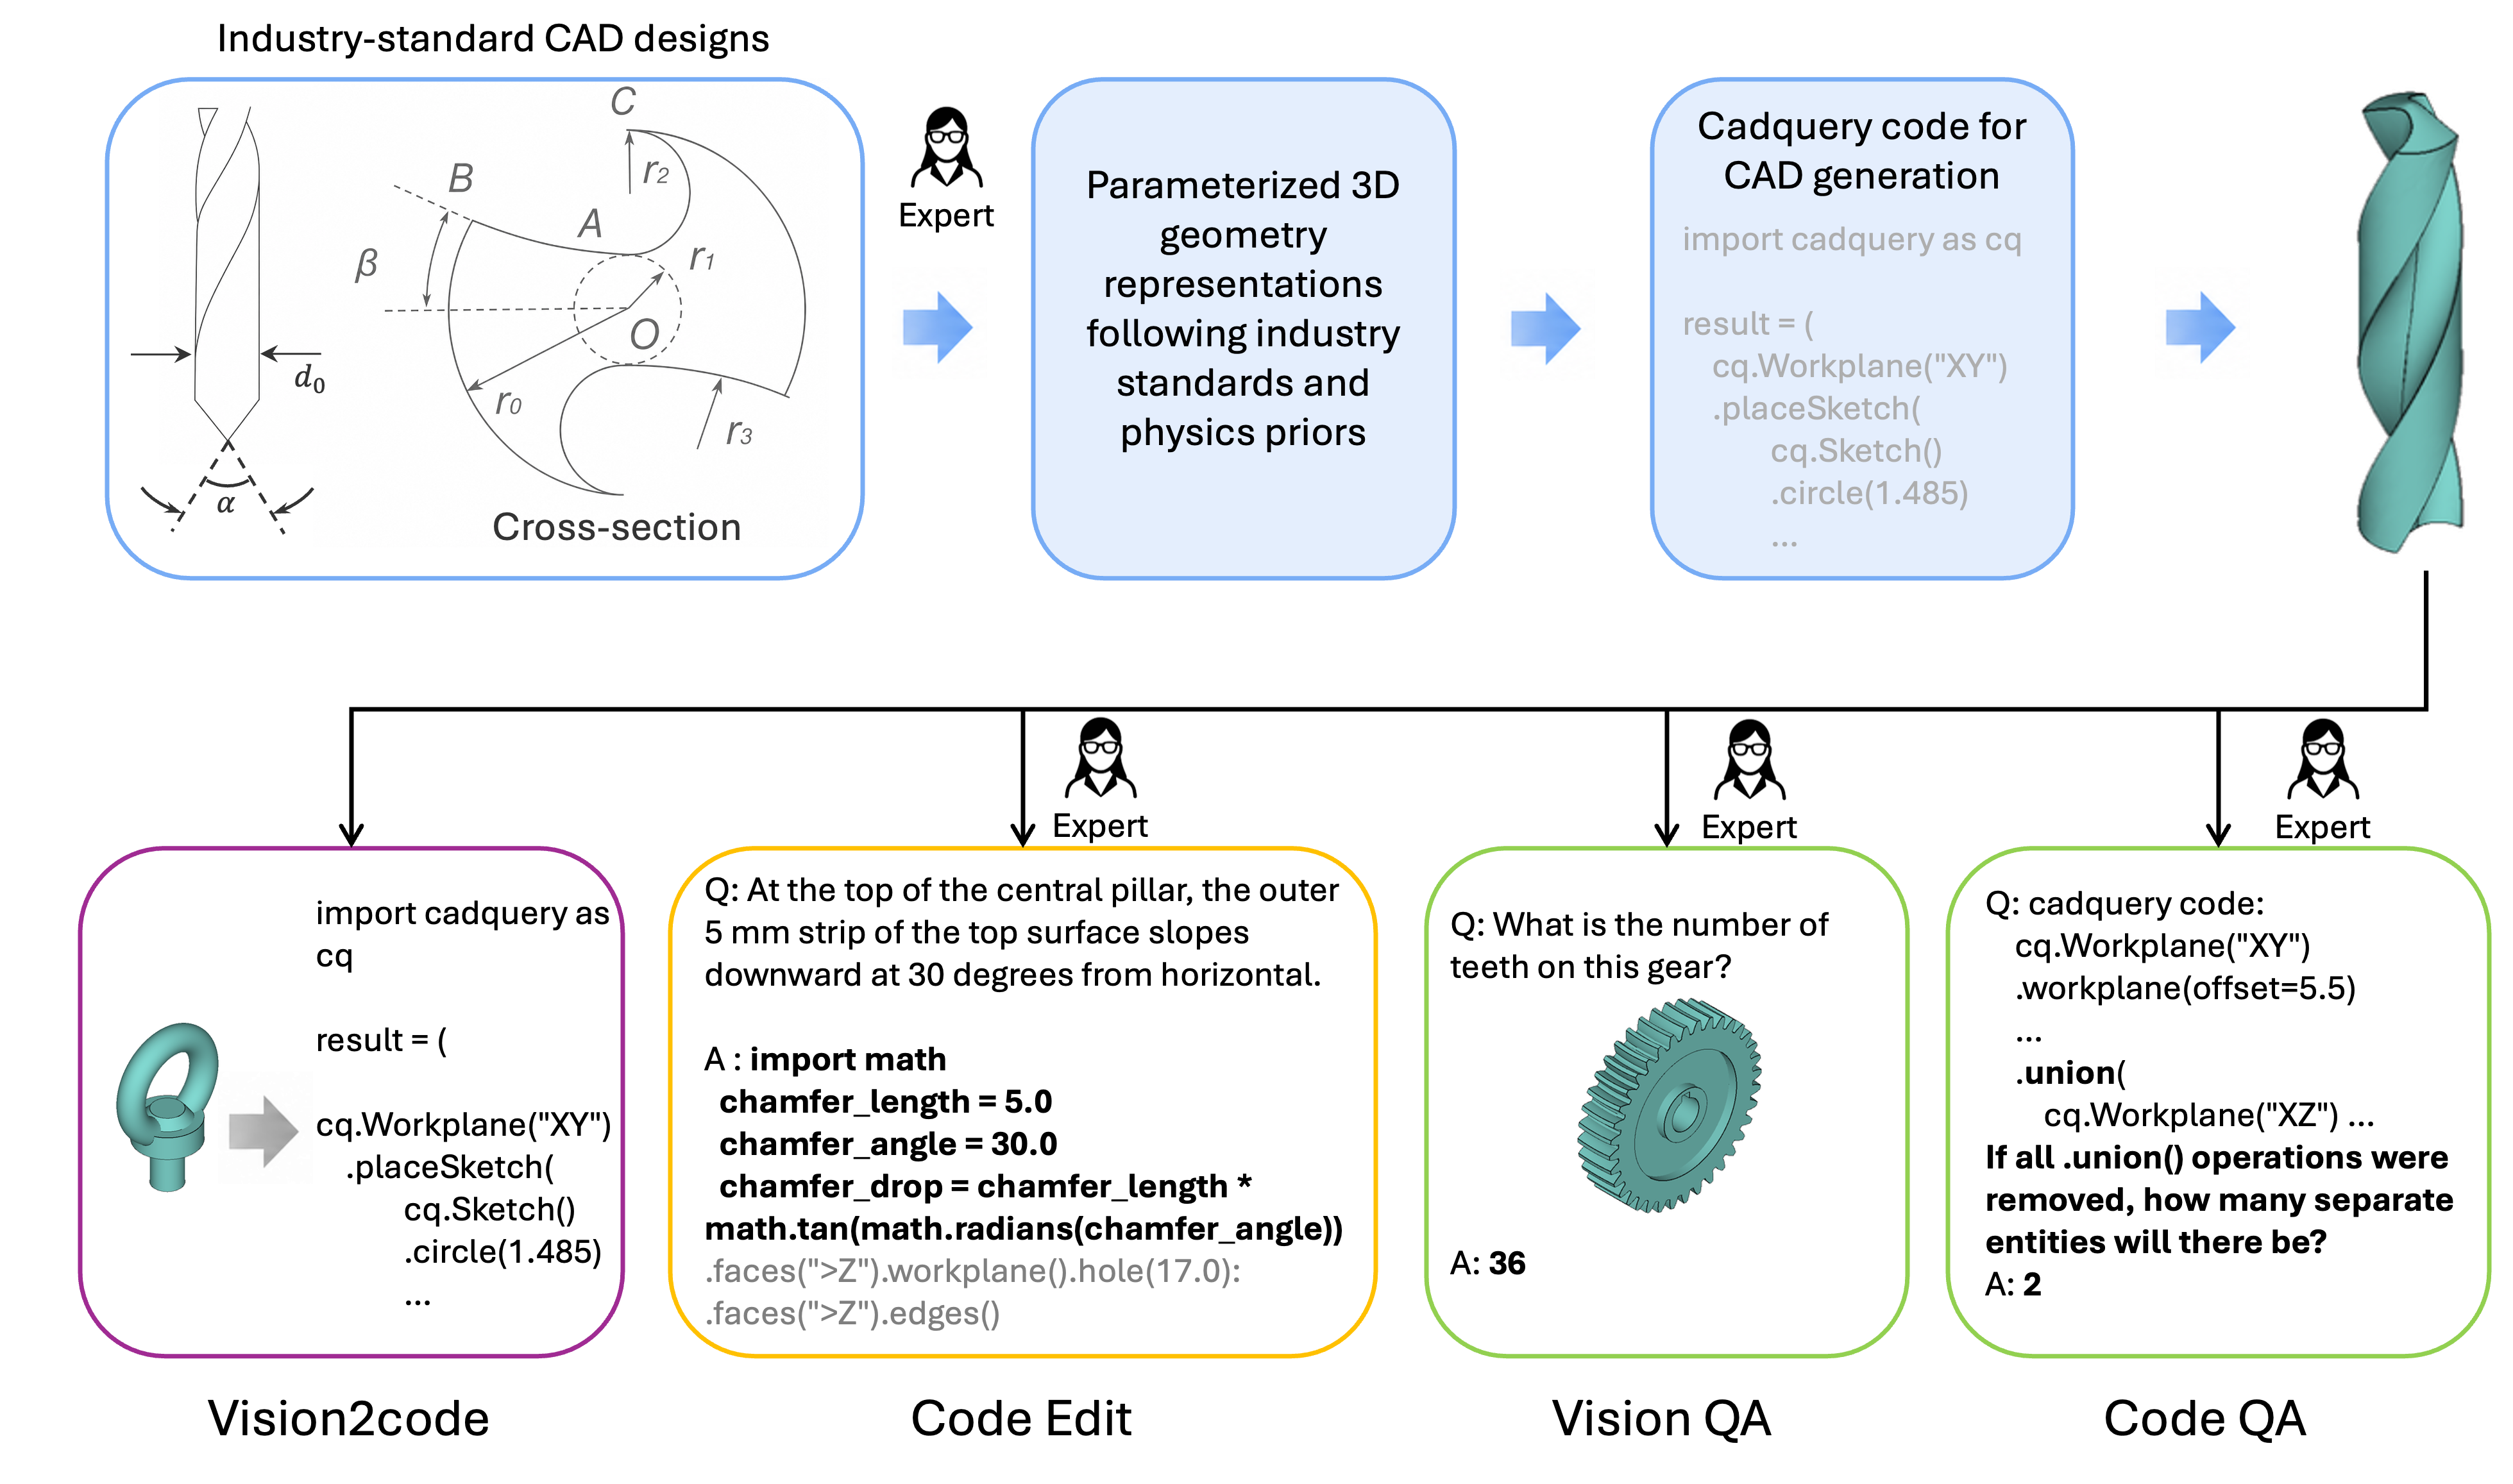
\includegraphics[width=\linewidth]{figures/fig_1.png}
  \caption{\textbf{BenchCAD overview.}
    BenchCAD evaluates multimodal models on executable and editable CAD reasoning across four tasks:
    image-to-CadQuery generation, code editing, image-based design QA, and code-based design QA.}
  \label{fig:teaser}
  \vspace{-1.8em}
\end{figure*}

Recent multimodal large language models (MLLMs) have begun to combine visual perception, code generation, and multi-step reasoning in a single interface.
This progress raises a natural question: can such models move beyond recognizing visual content to producing executable programs that define and modify physical objects?
Computer-aided design (CAD) provides a canonical setting for this question.
Unlike a mesh, point cloud, or rendered image, a CAD model is typically an editable parametric program: geometric operations such as extrusion, cutting, sweeping, filleting, and patterning construct a solid object through variables and constraints.
A capable CAD agent therefore requires more than visual recognition or code completion alone; it must connect visual evidence, 3D structure, symbolic operations, and executable program synthesis.

This makes CAD a promising application domain for MLLMs.
A useful CAD assistant should be able to read multi-view images or engineering sketches, infer the underlying 3D structure, answer design questions, generate executable CAD code, and edit existing programs while preserving unrelated geometry.
At the same time, CAD is also a challenging testbed for general AI capabilities.
Real designs are rarely arbitrary shapes.
They often belong to reusable families such as gears, springs, brackets, fasteners, pipes, and bearings, where small local details and parameter relations determine whether a part is merely visually similar or actually useful as an editable design.
For example, a spring is not fully specified by its helical silhouette; its end coils, pitch profile, and cross-section encode important design intent.
Similarly, a gear-like outline is insufficient without the correct tooth construction and parameterization.
In this sense, a model may produce geometry that passes the eye but fails the caliper.

Existing evaluations capture only parts of this problem.
3D and spatial reasoning benchmarks test whether models understand objects and viewpoints from images or code.
CAD code-generation benchmarks evaluate whether models can synthesize programs whose rendered outputs match a target shape, often using geometric metrics such as IoU or Chamfer distance.
Other datasets study program editing or design question answering in isolation.
However, these evaluations do not fully reveal whether a model has recovered the underlying parametric design logic: the part family, the construction operations, the dimensions and constraints, and the features that should remain invariant under edits.
A single end-to-end geometry score can therefore overestimate capability, because two programs may produce roughly similar outer envelopes while differing substantially in editability, operation choice, and engineering detail.

We ask: how should we evaluate whether MLLMs have the capabilities needed for practical CAD agents?
Such an evaluation should not only measure final shape similarity.
It should decompose the full CAD reasoning process into interpretable capabilities: recognizing the part and its 3D structure, understanding CAD operations, abstracting parameters and design constraints, synthesizing executable code, answering design questions, and applying localized edits without damaging non-target geometry.
This decomposition is important because failures in CAD are often compositional.
A model may identify the object family but choose the wrong operation, infer the rough scale but miss a standard relation, or edit the requested feature while unintentionally changing the rest of the part.

To address this gap, we introduce \textbf{BenchCAD}, a capability-decomposed benchmark for executable, editable, and constraint-aware CAD reasoning.
BenchCAD contains 17{,}900 execution-verified CadQuery programs across 106 industrial part families and 47 ISO/DIN/EN/ASME/IEC standards.
The dataset covers common reusable designs such as twist drills, bevel gears, compression springs, propellers, brackets, flanges, eye bolts, and fasteners.
Rather than sampling unconstrained primitive shapes, BenchCAD instantiates structured part families with meaningful parameter relations, standard-derived dimensions, and diverse CAD operations.
This allows the benchmark to test whether models can recover not only what a part looks like, but also how it should be constructed as an editable parametric program.

BenchCAD evaluates three practical CAD-agent workflows through four task families.
First, \texttt{img2cq} tests image-to-code generation: models must synthesize executable CadQuery programs from multi-view renders.
Second, \texttt{qa\_img} and \texttt{qa\_code} test design question answering from visual and program inputs, respectively, allowing us to diagnose whether failures arise from visual recognition, code understanding, operation reasoning, or parameter abstraction.
Third, \texttt{edit\_code} tests instruction-guided program editing, where the model must implement a requested local change while preserving unrelated geometry.
Together, these tasks turn CAD evaluation from a single shape-matching problem into a structured assessment of visual grounding, program synthesis, parametric reasoning, and edit preservation.

Across 10+ frontier MLLMs and open CAD-specialized baselines, BenchCAD reveals a consistent gap between apparent geometric similarity and true parametric understanding.
Current models often recognize the global part family but miss local engineering details, choose simplified or incorrect CAD operations, or fail to preserve non-target geometry during edits.
The comparison between image-based and code-based QA further shows that visual recognition alone does not imply reliable parametric abstraction.
Finally, our supervised fine-tuning (SFT) and reinforcement learning (RL) experiments show that training on BenchCAD improves operation coverage and executable generation, but substantial out-of-distribution gaps remain, especially for held-out industrial families requiring advanced operations and precise design constraints.

\paragraph{Contributions.}
Our contributions are threefold.
(i) We introduce \textbf{BenchCAD}, a domain-expert-verified dataset and generation pipeline containing 17{,}900 executable CadQuery programs across 106 industrial part families and 47 standards, together with multi-view renders, design QA pairs, and curated edit examples.
(ii) We propose a \textbf{unified CAD-agent evaluation framework} covering image-to-code generation, image/code-based QA, and instruction-guided code editing, with metrics that assess both target-task success and preservation of non-target geometry.
(iii) We provide a \textbf{capability-decomposed evaluation} of frontier MLLMs and open CAD-specialized models, showing that current systems remain limited by local detail recognition, CAD operation reasoning, parametric abstraction, and preservation-aware editing.
All data and code are anonymously released under \texttt{BenchCAD/cad\_bench} on Hugging Face under CC-BY-4.0.
\section{Related Work}
\label{sec:related}

\paragraph{Command-sequence CAD generation.}
The first wave of programmatic CAD generation operates on \emph{command-sequence representations} of sketch-and-extrude operations. DeepCAD~\citep{Wu2021} introduces a 178K-model corpus of Onshape parts encoded as discrete operation tokens, and Text2CAD~\citep{Khan2024} extends DeepCAD with 660K natural-language annotations spanning four abstraction levels, training a BERT-conditioned autoregressive transformer to emit those tokens. CAD-Coder~\citep{Guan2025} reformulates the same underlying data as CadQuery Python source and applies SFT + GRPO with a chain-of-thought prefix and Chamfer-distance reward, reaching mean CD $6.54\!\times\!10^{-3}$ on the Text2CAD test split.

\paragraph{The CadQuery-VLM lineage.}
A parallel research program has driven the recent state of the art in CadQuery code generation through three iterative releases. CAD-Recode~\citep{Rukhovich2025} first established the CadQuery formulation for reverse engineering, fine-tuning a Qwen2-1.5B language model on a procedurally generated corpus of 1M sketch-and-extrude scripts and reporting mean Chamfer distance 0.30 and IoU 92.0 on DeepCAD. cadrille~\citep{Kolodiazhnyi2026} extends this base by upgrading to Qwen2-VL-2B and unifying point-cloud, multi-view image, and text inputs in a single model, then introducing online reinforcement learning via Dr.CPPO with a piecewise IoU reward; the resulting cadrille-RL reaches DeepCAD image IoU 92.2 and Fusion360 image IoU 84.6 with 0.0\% invalidity. CADEvolve~\citep{Elistratov2026} shares the same backbone and RL recipe but expands the training corpus to 2.7M scripts via a GPT-5-mini-driven evolutionary loop, achieving DeepCAD image IoU 92.6. All three release model weights and inference scripts under permissive licences; we evaluate the latter two on BenchCAD as transfer baselines (\S\ref{sec:transfer}). These works collectively demonstrate the viability of CadQuery as a generation target and establish $\sim$92\% IoU as the saturated ceiling on existing benchmarks. They share three structural limitations BenchCAD addresses: training data is dominated by sketch+extrude operations, evaluation lacks both family-level taxonomy and standard-table grounding, and none decouple sub-capabilities --- every prior benchmark scores a single end-to-end metric, conflating visual perception, geometric abstraction, and code synthesis.

\paragraph{CAD code-generation and editing benchmarks.}
CADCodeVerify~\citep{Alrashedy2025} introduces \textbf{CADPrompt}, the first quantitative CAD code-generation benchmark --- 200 natural-language prompts paired with expert CadQuery code, scored via point-cloud distance and bounding-box IoU after ICP alignment. Despite establishing a useful protocol, CADPrompt is two orders of magnitude smaller than BenchCAD's verified split (20{,}143), lacks family taxonomy or difficulty stratification, leaks scale via absolute millimetre cues in prompts, and uses axis-aligned IoU that penalises geometrically correct but axis-permuted solutions. Beyond CADPrompt, two recent works target \emph{editing}: CAD-Editor proposes a locate-then-infill pipeline trained entirely on synthetic edit data without releasing a held-out human-verified edit benchmark, and CADialogue evaluates ten edit tasks within a conversational interface but does not release the eval set publicly. HistCAD~\citep{Dong2026} measures the preservation of ten geometric-constraint types (coincident, parallel, tangent) under edits via a FreeCAD edit-then-check protocol, but operates at the sketch-constraint level rather than at the executable-program level. To our knowledge, BenchCAD-Edit is the first public CAD benchmark with (i) execution-verified before/after CadQuery code pairs, (ii) a non-target preservation metric distinguishing target-feature success from program-wide locality, and (iii) cross-family balanced coverage with explicit edit-category taxonomy.

\paragraph{Vision-language spatial and code benchmarks.}
Recent benchmark methodology in adjacent domains informs our design. MMSI-Bench~\citep{MMSIBench2026} evaluates 37 multimodal LLMs on 1{,}000 hand-curated multi-image spatial reasoning questions across an 11-task taxonomy, reporting a 67-point human--model gap and showing that scaling model size yields negligible gains. AutoCodeBench~\citep{Chou2026} constructs a 3{,}920-problem multilingual code-generation benchmark via an automated LLM--sandbox pipeline and releases Lite/Complete subsets for differentiated evaluation regimes. Infinity-Chat~\citep{Hivemind2025} curates 26K real-world open-ended queries with 31K dense human annotations and reveals an ``Artificial Hivemind'' homogenisation effect across 70+ models. We adopt three of their structural patterns: explicit task taxonomy with per-task representatives (MMSI-Bench), Lite + Full split design for differentiated evaluation cost (AutoCodeBench), and a named, quantitative finding as the paper's punch line.

\paragraph{Position of BenchCAD.}
BenchCAD occupies a vacant intersection: a CAD code-generation benchmark that is simultaneously (i) \emph{execution-verified at scale} (20{,}143 parts at IoU $\geq 0.99$), (ii) \emph{standard-anchored} (55\% of families bound to ISO/DIN/EN/ASME/IEC specification tables), (iii) \emph{operation-rich} (45+ CadQuery operations versus 2--5 in prior corpora), and (iv) \emph{capability-decomposed} (five tasks isolating visual reconstruction, parametric abstraction, and code synthesis along the image$\to$code causal chain, including the first verified parametric edit task). Table~\ref{tab:cmp_prior} summarises this comparison.

\begin{table*}[t]
\centering
\small
\setlength{\tabcolsep}{5pt}
\caption{\textbf{BenchCAD versus prior CAD code-generation work.} BenchCAD is a \emph{unified, capability-decomposed evaluation framework} for large-model CAD reasoning, distinct in purpose from the CadQuery-VLM lineage (CAD-Recode, cadrille, CADEvolve) which releases training corpora alongside small fine-tuned models (Qwen 1.5B--2B) saturating $\sim$92\% IoU on legacy sketch+extrude splits. \textbf{Type:} \emph{C+M} = corpus+model, \emph{D} = dataset, \emph{B} = benchmark. \textbf{\#Fam.} = named industrial part families with explicit functional identity. \textbf{\#Std} = distinct ISO/DIN/EN/ASME/IEC specification codes. \textbf{\#Ops} = distinct CadQuery API methods exercised in the released corpus (static analysis of every released \texttt{.py}; see Appendix~\ref{app:ops}). \textbf{Adv} = all four advanced operation families (helix, loft/sweep, twist-extrude, parametric involute-gear) exercised. $\checkmark$ = supported, p.\ = partial, -- = absent.}
\label{tab:cmp_prior}
\begin{tabular}{lccrrrrccc}
\toprule
Benchmark & Yr & Type & \#Sam. & \#Fam. & \#Std & \#Ops & Adv & Edit & QA \\
\midrule
DeepCAD~\citep{Wu2021}                   & '21 & C+M & 178K  & -- & 0  & 4   & --   & --   & --   \\
Fusion360 G.~\citep{Willis2021fusion}    & '21 & D   & 8K    & -- & 0  & 6   & --   & --   & --   \\
Text2CAD~\citep{Khan2024}                & '24 & C+M & 170K  & -- & 0  & 17  & --   & --   & --   \\
CADPrompt~\citep{Alrashedy2025}          & '25 & B   & 200   & -- & 0  & --  & p.\  & --   & --   \\
CAD-Coder~\citep{Guan2025}               & '25 & C+M & 110K  & -- & 0  & 4   & --   & p.\  & --   \\
CAD-Recode~\citep{Rukhovich2025}         & '25 & C+M & 1M+7K & -- & 0  & 18  & --   & p.\  & seq.\\
cadrille~\citep{Kolodiazhnyi2026}        & '26 & C+M & 1M+7K & -- & 0  & 18  & --   & --   & --   \\
CADEvolve~\citep{Elistratov2026}         & '26 & C+M & 2.7M  & -- & 0  & 25  & p.\  & --   & --   \\
\midrule
\textbf{BenchCAD (ours)} & \textbf{'26} & \textbf{D+B} & \textbf{17{,}900} & \textbf{106} & \textbf{43} & \textbf{49} & $\checkmark$ & $\checkmark$ & $\checkmark$ \\
\bottomrule
\end{tabular}
\end{table*}

\section{The BenchCAD Dataset}
\label{sec:dataset}

\subsection{Design Principles}
We design BenchCAD around four principles that prior CAD datasets violate either individually or jointly.

\paragraph{P1 --- Execution as ground truth.} Every record's ground truth is the \emph{executed} solid: the CadQuery source code is run inside a sandboxed CadQuery / PythonOCC environment, the resulting STEP file is voxelised, and compared against a reference solid by 3D IoU under the rotation-invariant 6-face cube group~\citep{rot_iou}. A record enters the verified split only if IoU $\geq 0.99$ \emph{and} executes within a 30\,s timeout with non-degenerate volume. This rules out the silent failure mode common in DeepCAD-derived corpora where parsed code is assumed correct but neither re-executed nor geometrically validated.

\paragraph{P2 --- Standard-table anchoring.} Where a part has an industrial counterpart, parameters sample from real specification tables (ISO 22 V-belt cross-section series, DIN 338 twist-drill diameter ranges, ISO 23509 bevel-gear pitch--module relationship). Geometry that ``looks right'' but violates manufacturable proportions (e.g.\ M6 bolt with 3\,mm thread pitch) is rejected at sampling time. 55\% of BenchCAD families are standard-anchored; Table~\ref{tab:standards} enumerates the standard codes.

\paragraph{P3 --- Family-level taxonomy.} Records are grouped into 106 named families (e.g.\ \texttt{coil\_spring}, \texttt{helical\_gear}, \texttt{twisted\_drill}), each implemented by a small Python module exposing a typed parameter schema, a sampler, a validator, and a deterministic builder. This makes coverage measurable, sampling reproducible, difficulty controllable, and per-family analysis trivial --- properties absent from DeepCAD/Fusion360 where parts are pooled without semantic structure.

\paragraph{P4 --- Operation breadth.} The dataset exercises 45+ distinct CadQuery operations spanning sketch primitives, contour drawing (lines, arcs, splines), workplane manipulation, sketch arrays, 3D operations (extrude, twist-extrude, revolve, loft, sweep), Booleans, hole variants, and edge finishing (fillet, chamfer, shell). Appendix~\ref{app:ops} contrasts this against prior corpora restricted to sketch+extrude.

\subsection{Family Registry and Standard Compliance}
Each family is a class implementing the \texttt{Family} interface: a JSON-schema parameter spec; a \texttt{sample\_params(difficulty, rng)} method that draws a parameter dictionary; a \texttt{validate\_params(p)} predicate enforcing geometric and standard-table constraints; and a \texttt{make\_program(p)} method that emits a typed list of \texttt{Op} dicts consumable by the builder. Families are auto-discovered from a registry module; adding a new family requires no changes to the pipeline beyond registering one class. A family declares \texttt{standard = "ISO 23509"} (etc.) when its parameter ranges and inter-parameter relations are fixed by an external specification table. As of submission, BenchCAD covers 22 ISO codes (e.g.\ ISO 22, 113, 272, 1234, 2339, 2936, 10828, 23509), 28 DIN codes (e.g.\ DIN 338, 471/472, 580, 5480, 2095, 8187), 4 EN codes, 3 ASME codes, and 2 IEC codes --- totalling 59 standard-anchored families. The remaining 47 families cover bespoke industrial parts (e.g.\ \texttt{twisted\_bracket}, \texttt{venturi\_tube}, \texttt{lobed\_knob}) without formal standards but governed by analogous proportional rules.

Each family supports three difficulty tiers --- \emph{easy}, \emph{medium}, \emph{hard} --- defined by parameter complexity (op count, feature count, non-axis-aligned geometry, presence of helical, lofted, or boolean operations). Tier definitions are family-specific and machine-checkable; aggregate counts and tier example renders appear in Figure~\ref{fig:taxonomy}.

\begin{table}[t]
\centering
\small
\caption{\textbf{Standard-anchored families.} 55\% of BenchCAD families bind their parameters to ISO/DIN/EN/ASME/IEC specification tables, sampling at values drawn from real engineering ranges rather than arbitrary geometry. The bottom row lists the 47 custom families covering bespoke industrial parts (twisted brackets, lobed knobs) governed by analogous proportional rules without formal standards.}
\label{tab:standards}
\begin{tabular}{llr}
\toprule
Standard & Codes covered (sample) & \#Fam. \\
\midrule
ISO   & 22, 113, 272, 1234, 2339, 2936, 10828, 23509, \ldots & 22 \\
DIN   & 338, 471/472, 580, 5480, 2095, 8187, 71412, \ldots    & 28 \\
EN    & 10034, 10056, 10219, 10279                            & 4  \\
ASME  & B1.20.1, B16.5, B16.9                                 & 3  \\
IEC   & 60072-1, 60086                                        & 2  \\
\midrule
\textbf{Total standard-anchored}   &                              & \textbf{59 (55\%)} \\
Custom (no formal standard)        &                              & 47 \\
\bottomrule
\end{tabular}
\end{table}


\subsection{The CadGen Pipeline}
We name the data construction pipeline \textbf{CadGen} to separate it as a standalone contribution from the resulting dataset. CadGen has four stages.

\paragraph{Stage 1 --- Parameter sampling.} For each family $\times$ difficulty bucket, the sampler draws parameters from the JSON schema under standard-table constraints. Sampling is deterministic given a seed.

\paragraph{Stage 2 --- Program emission.} The family's \texttt{make\_program} returns an op sequence. The builder consumes the op list and produces (i) Python CadQuery source code via a per-op code template, and (ii) a CadQuery \texttt{Workplane} object via direct API dispatch. Both representations are aligned by construction: the same op list yields equivalent geometry whether interpreted via the builder or by executing the emitted code in a fresh sandbox.

\paragraph{Stage 3 --- Execution and verification.} We re-execute the emitted code in an isolated sandbox, export STEP, voxelise at 64$^3$ resolution, and compute rotation-invariant 3D IoU against the builder's direct STEP output. Records with IoU $< 0.99$, execution failures, timeouts ($>$30\,s), or zero/inverted volume are quarantined for review. A persistent execution cache avoids re-running the same code on subsequent syncs.

\paragraph{Stage 4 --- Render and package.} Each verified record is rendered to four canonical views (front / right / top / iso) at 512$\times$512 with VTK, and the (parameters, program, code, STEP, views) bundle is registered to the dataset CSV.

\paragraph{Yield.} From a 20{,}221-sample run on the April 2026 batch, 20{,}143 records (99.6\%) passed all checks; the 78 failures concentrated in three pathological families (\texttt{double\_simplex\_sprocket}, \texttt{stepped\_shaft}, \texttt{torus\_link}) due to OCCT \texttt{Standard\_Failure} on extreme parameter combinations.

\subsection{Splits, Documentation, and Hosting}
\paragraph{Splits.} The full release contains six subsets (Table~\ref{tab:dataset}): \emph{BenchCAD-Synth} (20{,}143 verified procedural parts, primary evaluation set); \emph{BenchCAD-Edit} (433 curated edit pairs spanning dimensional / additive / subtractive / multi-step modifications across 106 families); \emph{BenchCAD-Lite} (530-sample stratified subset for fast leaderboards); \emph{BenchCAD-Fusion360} and \emph{BenchCAD-DeepCAD} (verified subsets for OOD evaluation); and \emph{BenchCAD-GenCAD} (162{,}000 image-to-code pairs derived from GenCAD~\citep{GenCAD2025} for SFT-scale training).

\paragraph{Documentation, hosting, licence.} Every dataset ships with a Croissant 1.0 metadata file including all required Responsible AI fields. Validation passes the public Croissant checker. All splits are hosted on Hugging Face under \texttt{BenchCAD/cad\_bench} (test) and \texttt{BenchCAD/cad\_bench\_edit} (edit), with the verification-pipeline source under MIT and the dataset under CC-BY-4.0. Dataset cards link to per-family parameter schemas and the standard-table sources used for compliance. A datasheet following~\citet{rot_iou} appears in Appendix~\ref{app:datasheet}.

\begin{table}[t]
\centering
\small
\caption{\textbf{BenchCAD dataset composition.} Three released datasets: the verified CadQuery code core (17{,}900 parts spanning 106 families, each with parametric source, executable STEP, four canonical-view renders, parameter JSON, and op list), the paired QA bank (2{,}400 questions evaluated under both visual and code conditioning), and the Edit subset (748 before/after pairs).}
\label{tab:dataset}
\begin{tabular}{lrrl}
\toprule
Dataset & \#Records & \#Families & GT artefacts \\
\midrule
BenchCAD                     & 17{,}900             & 106 & code $\cdot$ STEP $\cdot$ 4 views $\cdot$ params $\cdot$ ops \\
BenchCAD-QA (paired img/code)& 2{,}400 $\times 2$   & 106 & question $+$ gold answer \\
BenchCAD-Edit                & 748                  & 106 & before/after $+$ NL instruction \\
\bottomrule
\end{tabular}
\end{table}


\begin{figure}[t]
  \centering
  \fbox{\rule[-2cm]{0cm}{4cm} \rule[0cm]{14cm}{0cm}}
  \caption{\textbf{BenchCAD overview.} (Top-left) sample parts from four families, with the formula-driven parametric structure highlighted (involute equation for gears, helix parametric for springs, ISO 23509 module--tooth--pitch relation for bevel gears). (Top-right) the 106-family taxonomy split by standard body (ISO/DIN/EN/ASME/IEC/custom). (Bottom-left) the five evaluation tasks and their capability coverage. (Bottom-right) headline finding: image-conditioned QA trails code-conditioned QA by 15--20\,pt across all 30+ evaluated models (Vision Bottleneck). \emph{Placeholder figure --- replace with composed PDF.}}
  \label{fig:overview}
\end{figure}

\begin{figure}[t]
  \centering
  \fbox{\rule[-2cm]{0cm}{4cm} \rule[0cm]{14cm}{0cm}}
  \caption{\textbf{Family taxonomy and difficulty stratification.} Each row shows three representative parts (easy / medium / hard) drawn from a single family. Difficulty tiers are family-specific and machine-checkable; complexity grows along (a) op count, (b) feature count, (c) presence of helical/lofted/boolean operations. \emph{Placeholder figure --- replace with composed PDF.}}
  \label{fig:taxonomy}
\end{figure}

\section{Experiments}
\label{sec:experiments}

\subsection{Setup} 
\label{sec:exp_setup}
We evaluate 10+ models with non-uniform per-task coverage; the headline figures (Fig.~\ref{fig:main_results}) report seven frontier proprietary systems with full four-task coverage --- \textbf{GPT-4o}, \textbf{GPT-5.3} (think / non-think), \textbf{Claude Opus 4.7} (think / non-think), \textbf{Gemini 3.1 Pro} (think / non-think) --- with open-source baselines (Qwen2.5-VL, InternVL3) and CAD-specialised cadrille-RL on subsets.
For each task, we include a \emph{blind baseline} and evaluate model capabilities by quantifying the performance gains of each model over the baseline across all relevant metrics.
%Inference at temperature 0 with a 60\,s per-sample budget; open models on 8$\times$A800-80GB, proprietary via API.
%We include a \emph{blind baseline} and an \emph{Oracle} reference (GT-code parameter substitution; trivially 100\%).
%Headline numbers use BenchCAD (530 stratified samples); per-model per-task coverage and the full 17{,}900-set scores for the top systems are in Appendix~\ref{app:full_results}.

\subsection{Main Results}
\label{sec:exp_main}

\begin{wrapfigure}{r}{0.5\linewidth} % r=right, width=50% of line
  \vspace{-20pt} % 可选：微调与上方文字的间距
  \centering
  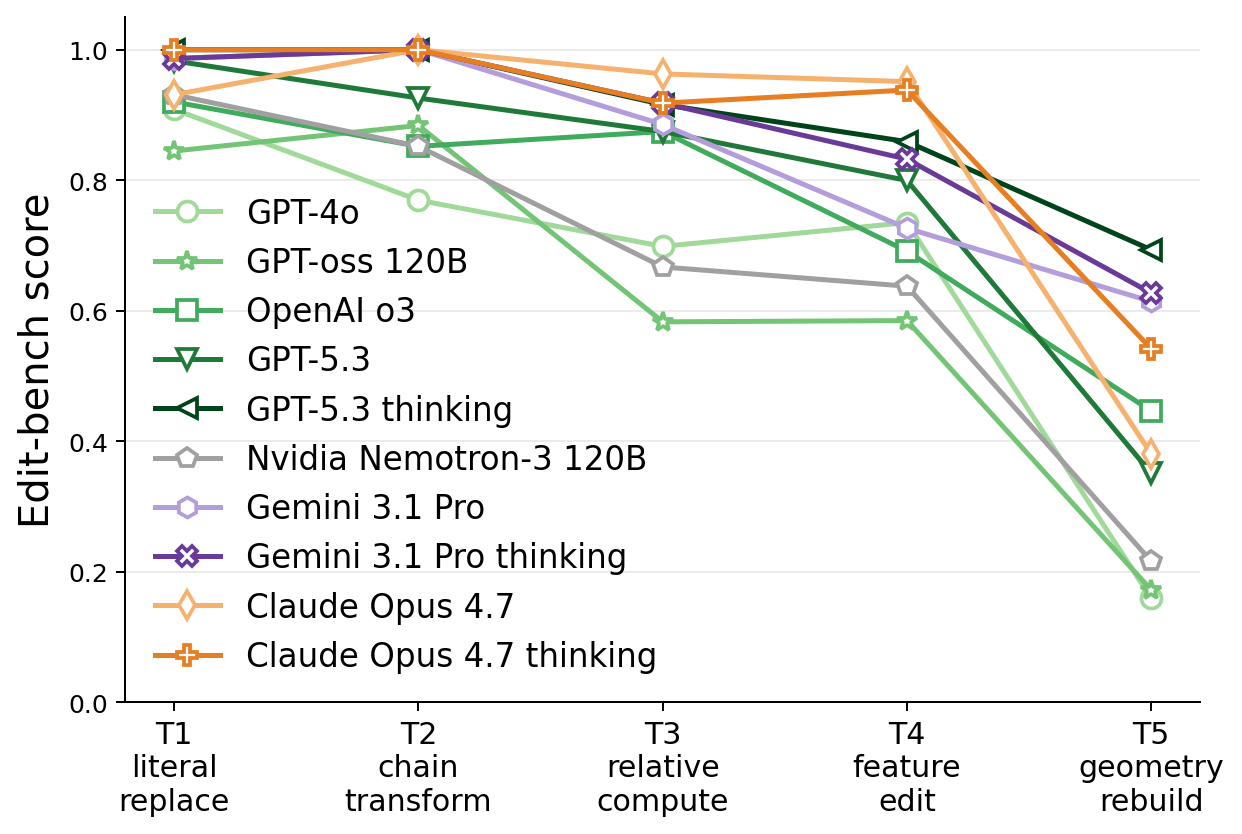
\includegraphics[width=0.9\linewidth]{figures/fig_5.png}
  \caption{\textbf{BenchCAD-Edit by task type.} }
  \label{fig:edit_task}
  \vspace{-10pt} % 可选：微调与下方文字的间距
\end{wrapfigure}

Table~\ref{tab:main_eval_qa_img} indicates that Vision QA remains challenging for current frontier MLLMs. Performance is relatively stronger on Holistic Visual Recognition and Spatial / Code Reasoning, but consistently weaker on CAD Operation Understanding and Industrial Parametric Abstraction, suggesting that models can often recognize global shapes while still struggling to infer CAD operations and parametric design intent. Moreover, thinking mode does not consistently improve performance, because extended reasoning can amplify hallucinations about geometric structures, dimensions, or CAD operations. These results suggest that CAD QA requires more than generic reasoning ability; it demands precise visual grounding, CAD-specific knowledge, and robust parametric abstraction.





Table~\ref{tab:main_eval_qa_code} shows that direct access to CadQuery code substantially improves QA performance compared with the vision-conditioned setting in Table~\ref{tab:main_eval_qa_img}.
The best models achieve total scores around 0.84, far above the best visual-conditioned score of 0.587. 
This large modality gap suggests that current MLLMs are considerably better at extracting geometric and parametric information from explicit CAD programs than from rendered images. 
However, performance on Spatial / Code Reasoning remains comparatively lower, indicating that code access alone does not fully resolve the need for precise spatial and operational reasoning.

The Vision2Code leaderboard (Table~\ref{tab:codegen_unified}) shows three patterns:
(i) the specialist CAD lineage transferred from DeepCAD scores poorly on BenchCAD (Cadrille-RL total 0.338, CADEvolve v3 0.601);
(ii) frontier MLLMs cap mid-range (gemini-3.1-pro-thinking total 0.318) and exhibit non-monotonic thinking-mode behaviour;
(iii) our open Qwen3-VL-2B trained on BenchCAD reaches total 0.628 (iid-sft) and 0.723 (ood-sft$+$RL, best overall) --- showing the dataset is learnable on a small backbone and that RL meaningfully closes the generalisation gap.

\begin{table}[t]
\centering
\small
\setlength{\tabcolsep}{6pt}
\renewcommand{\arraystretch}{1.05}
\caption{\textbf{Vision2Code unified leaderboard.} Specialist CAD lineage (cadrille / CADEvolve), frontier MLLMs, and our open Qwen3-VL-2B trained baseline. All BenchCAD scores on BenchCAD-Lite. \emph{(\,$\dagger$\,)} Ours-SFT-IID is evaluated on the IID split (all 106 families seen at train time); all other rows are OOD on BenchCAD by construction (specialist lineage and frontier MLLMs never saw BenchCAD; ours-SFT-OOD / +RL hold out 10 mech.-transmission families). Essential-op recall is the fraction of ground-truth essential operations (helix / sweep / loft / twist-extrude / parametric involute-gear) recovered by the prediction.}
\label{tab:codegen_unified}
\begin{tabular}{@{}lcccl@{}}
\toprule
Model                                                  & DeepCAD IoU      & BenchCAD IoU            & Ess.\ op recall  & Notes \\
\midrule
\multicolumn{5}{l}{\emph{Specialist CAD lineage ($\sim$2B, OOD on BenchCAD)}} \\
cadrille-RL~\citep{Kolodiazhnyi2026}                   & 0.919            & 0.273                   & --               & sketch+ext, 1M \\
CADEvolve~\citep{Elistratov2026}                       & 0.923            & 0.039                   & --               & extended, 2.7M \\
\midrule
\multicolumn{5}{l}{\emph{Frontier MLLMs (BenchCAD-Lite, by def.\ OOD)}} \\
gpt-4o                                                 & --               & 0.188                   & 0.468            & \\
gpt-5.3 (thinking)                                     & --               & 0.207                   & 0.455            & \\
claude-opus-4.7 (thinking)                             & --               & 0.267                   & 0.471            & \\
gemini-3.1-pro (thinking)                              & --               & \textbf{0.279}          & \textbf{0.567}   & strongest frontier \\
\midrule
\multicolumn{5}{l}{\emph{Ours --- Qwen3-VL-2B, 9 GPU-h on $8{\times}$A800-80GB}} \\
SFT (IID, 106 fam.\ seen)$^{\dagger}$                  & --               & \textbf{0.650}          & \textbf{0.950}   & dataset learnable on 2B \\
SFT (OOD, 10 fam.\ held out)                           & --               & 0.180                   & 0.200            & generalisation gap \\
\quad $+$ RL ($r{=}0.2\,\mathrm{ess}{+}0.8\,\mathrm{IoU}$) & --             & 0.350                   & 0.450            & RL partial recovery \\
\bottomrule
\end{tabular}
\end{table}


% Table~\ref{tab:main_eval} reports per-task accuracy and the macro-mean.
% The strongest model overall is GPT-5.3 (think) at 46.8\% Avg --- well below the IoU $\geq 0.99$ verification threshold and leaving substantial room across every task.
% Three observations stand out.
% \textbf{Absolute scores remain low}: even top reasoning models score below 50\% on every task; the strongest open-source VLM (Qwen2.5-VL-72B, 23.5\% Avg) trails the best proprietary system by 23\,pt; CAD-specialised text/point-cloud models (CAD-Coder-7B, CAD-Recode-1.5B) sit between mid-tier proprietary and top-tier open-source on their applicable tasks despite matching the latter on the original DeepCAD benchmark.
% \textbf{Scaling is not enough}: InternVL3 1B$\to$78B raises Avg by only 14.5\,pt over a 78$\times$ parameter expansion; Qwen2.5-VL 7B$\to$72B by only 7.5\,pt.
% \textbf{Geometry-program decoupling}: several mid-tier models (Gemini 3.1 Pro, GPT-4o) achieve respectable IoU on \texttt{img2cq} but mid-tier scores on \texttt{qa\_img}, indicating they recover the outer shape but cannot answer dimensional questions about it.

% tab_main_eval moved to Appendix~\ref{app:full_results}

\begin{figure*}[t]
  \centering
  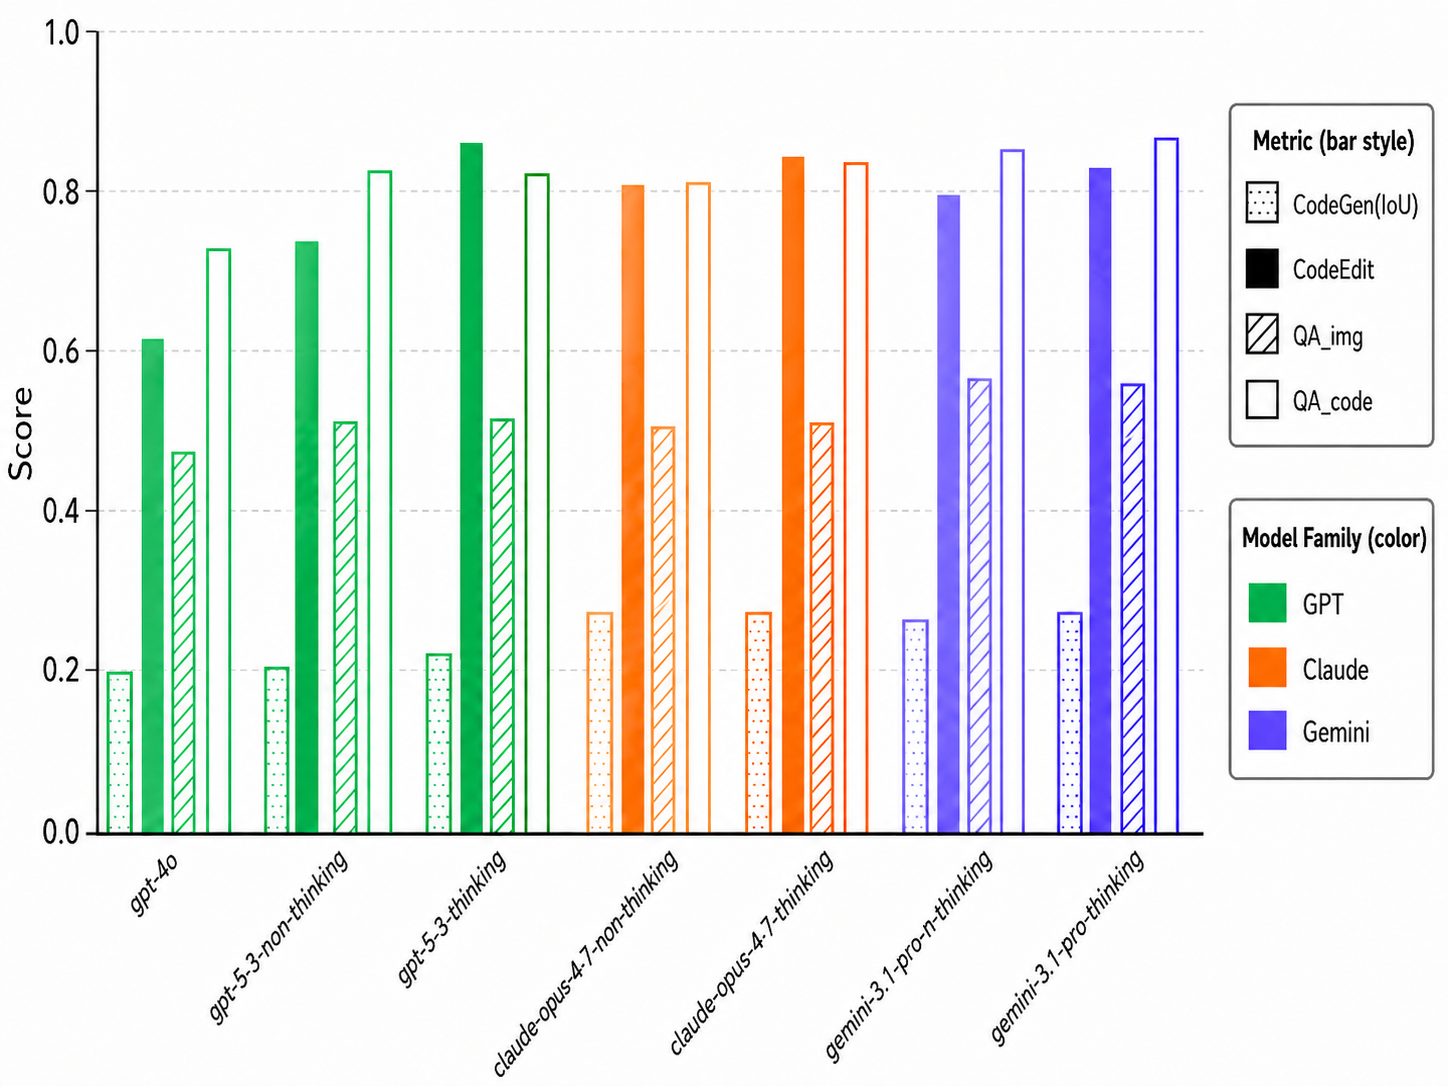
\includegraphics[width=0.65\linewidth]{figures/fig_3.png}
  \caption{\textbf{Per-model performance across the four BenchCAD task categories} (frontier proprietary subset; open-source baselines in Table~\ref{tab:main_eval_qa_img}). Bar style encodes task; colour encodes model family; within-family variants distinguish thinking vs.\ non-thinking. Two patterns motivate the diagnostics that follow: (i) QA-img is consistently lower than QA-code (\emph{Holistic Spatial and Detailing Deficit}, \S\ref{sec:exp_failure_analysis}), and (ii) CodeEdit trails CodeGen on every model, reflecting \emph{Industrial Common Sense Gap} (\S\ref{sec:exp_edit}).}
  \label{fig:main_results}
\end{figure*}


\subsection{Failure Analysis}
\label{sec:exp_failure_analysis}

Building on the layered evaluation introduced in \S\ref{sec:capability}, we examine four representative \textsc{Vision2Code} failures elicited from frontier reasoning models on hard-tier families, each diagnostic of a different level in the capability hierarchy.

\textbf{$L_1$ --- holistic feature recognition.} A hex-head bolt is reproduced with the correct overall body but with its threaded shank and DIN-standard head detail omitted. The vision encoder integrates the global silhouette while failing to register the high-information local features that distinguish a manufacturable bolt from a smooth pin --- a deficit at the perception layer rather than at code generation.

\textbf{$L_1$ --- spatial understanding.} On a bearing retainer cap, the 24-axis rotation-invariant IoU is substantially higher than the single-axis IoU --- a diagnostic signature that the generated geometry is approximately correct but oriented on the wrong base workplane. Inspecting the emitted code confirms it: the model defaults to the XY plane that dominates its training distribution and fails to recognise that the part is naturally extruded along XZ. This is a perception failure at the spatial-anchoring layer rather than a geometric or symbolic one, and one that no amount of code-side reasoning can recover.

\textbf{$L_2$ --- operation understanding.} A twisted bracket is generated as a flat plate with mounting holes; the requisite twist-extrusion is absent from the emitted program entirely. The model recognises the part outline at $L_1$ but fails to map the visible torsion to the corresponding CAD operation, exposing an Op Vocabulary Gap (\S\ref{app:op_gap_full}) at the operation-understanding layer.

\textbf{$L_3$ --- parametric abstraction.} A coil spring with non-uniform pitch is reproduced as a uniform helix. The model recognises the spring family at $L_1$ and emits a helical sweep at $L_2$, yet flattens the pitch profile from variable to constant --- losing the parametric structure that an engineer would have written explicitly. This is an $L_3$ failure invisible to either $L_1$ or $L_2$ metrics, and it is precisely the class of failure that motivates anchoring BenchCAD families to ISO/DIN/EN/ASME/IEC standards.

These cases illustrate how the layered framework converts \textsc{Vision2Code} failures from a single opaque ``wrong code'' category into level-attributable diagnostics: a model can succeed at $L_1$ yet fail at $L_2$ (the bracket), or succeed at $L_1$ and $L_2$ yet fail at $L_3$ (the spring). Without per-level attribution these distinctions collapse into a single low IoU score, and the corresponding training signal --- which level to strengthen --- is lost.

% \subsection{Holistic Spatial and Detailing Deficit and Capability Profile}
% \label{sec:exp_capability}

% The framework of \S\ref{sec:capability} predicts that the gap between \texttt{qa\_img} and \texttt{qa\_code} on matched prompts isolates $L_1$ (Holistic Visual Recognition) from $L_2$ (CAD Operations Understanding).
% Table~\ref{tab:main_eval_qa_img} shows this gap is large and remarkably consistent: 19.6\,pt for GPT-5.3, 19.8\,pt for Claude Opus 4.7, 16.9\,pt for GPT-4o, 12.9\,pt for Qwen2.5-VL-72B.
% We name this the \textbf{Holistic Spatial and Detailing Deficit}.
% It is robust along three axes: it survives chain-of-thought (reasoning variants show the largest absolute gap), survives view-count augmentation (4$\to$8 views recovers $\leq$1.5\,pt; Appendix~\ref{app:ablation}), and survives parameter scaling within open-source families (the relative gap is preserved as absolute scores collapse).
% These properties suggest the Holistic Spatial and Detailing Deficit is a property of the \emph{representation interface} between vision encoders and language decoders, not of any single model's capacity.

% A per-model capability profile across six axes (surface similarity, local feature accuracy, global geometry, CAD understanding, CAD code robustness, synthesis) and four recurring failure modes (\emph{no industry understanding}, \emph{wrong plane}, \emph{wrong ops}, \emph{no detail}) appear in Appendix~\ref{app:capability_profile} (Figure~\ref{fig:capability_profile}); frontier models occupy structurally different capability shapes (GPT-5.3 leads on CAD understanding and code robustness, Claude Opus 4.7 on local feature accuracy and synthesis, Gemini 3.1 Pro on global geometry), confirming that no single model dominates all axes.

\subsection{The Family Cliff}
\label{sec:exp_cliff}

Table~\ref{tab:family_cliff} stratifies \texttt{img2cq} pass rate by family difficulty tier.
The strongest model collapses by 48\,pt from easy (68\%) to hard (20\%), exhibiting a \textbf{Family Cliff} attributable to two interacting factors: hard-tier families exercise advanced operations (helical sweeps, twist-extrusion, lofted Booleans) that scarcely appear in any prior CAD training corpus, and they enforce non-trivial parametric constraints (gear module--tooth--pitch consistency, spring free-length--turn-count coupling) that no model evaluated reliably preserves.
The cliff persists across architectures: closed-source post-training quality dominates the easy-tier gap (Qwen2.5-VL-72B trails GPT-5.3 by 30\,pt on easy) but converges on hard (15\,pt gap) because both models hover near the floor.

% tab_family_cliff moved to Appendix~\ref{app:full_results}

\subsection{The Edit Task: Verified Parametric Editing}
\label{sec:exp_edit}

\paragraph{Setup.} BenchCAD-Edit comprises 748 verified $(\text{original}, \text{instruction}, \text{target})$ triples balanced across all 106 families and stratified into five task types: T1 \emph{literal\_replace}, T2 \emph{chain\_transform}, T3 \emph{relative\_compute}, T4 \emph{feature\_edit}, T5 \emph{geometry\_rebuild} (Table~\ref{tab:task_taxonomy}, Appendix~\ref{app:edit_protocol}). Targets pass through the same expert-verified construction pipeline used for BenchCAD (\S\ref{sec:dataset}).

\paragraph{Metrics.} For a model prediction with rendered solid $S_g$, original solid $S_o$, and target solid $S_t$, let $\mathrm{IoU}(S_a, S_b)$ denote the voxel intersection-over-union at $64^3$. Over $n$ records (failed executions count as zero IoU) we report four pass@1 metrics:
\begin{align}
\mathrm{exec\_rate} &= \tfrac{1}{n}\textstyle\sum_i \mathbf{1}[\,\text{prediction}_i\ \text{ran}\,], \label{eq:exec}\\
\mathrm{strict\_rate} &= \tfrac{1}{n}\textstyle\sum_i \mathbf{1}[\mathrm{IoU}(S_g^i, S_t^i) \geq 0.99], \label{eq:strict}\\
\mathrm{mean\_iou}   &= \tfrac{1}{n}\textstyle\sum_i \mathrm{IoU}(S_g^i, S_t^i), \label{eq:miou}\\
\mathrm{mean\_norm}  &= \tfrac{1}{|\mathcal{N}|}\textstyle\sum_{i \in \mathcal{N}} \mathrm{clip}\!\left(\tfrac{\mathrm{IoU}(S_g^i, S_t^i) - \mathrm{IoU}(S_o^i, S_t^i)}{1 - \mathrm{IoU}(S_o^i, S_t^i)},\,0,\,1\right), \label{eq:norm}
\end{align}
where $\mathcal{N} = \{i : \mathrm{IoU}(S_o^i, S_t^i) \leq 0.99\}$ excludes degenerate records on which the original is already at the target. \texttt{mean\_norm} is a headroom-normalised improvement: $1$ means the model fully traversed the original-to-target gap, $0$ means it did not move at all. All metrics are pass@1: a single API call per (record, model) with no resampling. A complementary 6-orientation rotation-invariant voxel IoU is computed alongside the standard IoU and used only for failure attribution (\S\ref{sec:exp_failure_analysis}, \emph{wrong-plane} diagnostic).

\paragraph{Models.} We score ten code LLMs spanning 2024--2026: \texttt{gpt-4o} (OpenAI, 2024), \texttt{o3} (OpenAI, 2025), \texttt{gpt-oss-120b} (OpenAI open-weights, 2025), \texttt{gpt-5.3-chat-latest} with and without \texttt{reasoning=medium} (OpenAI, 2025--26), \texttt{nemotron-3-super-120b-a12b} (NVIDIA, 2026), \texttt{gemini-3.1-pro-preview} with and without thinking (Google DeepMind, 2026), and \texttt{claude-opus-4-7} with and without \texttt{reasoning=high} (Anthropic, 2026). Closed models are queried through their official APIs; open-weights models via OpenRouter.


  \paragraph{Findings.} Table~\ref{tab:main_results} ranks the ten models by \texttt{mean\_norm}; Figure~\ref{fig:edit_task} disaggregates performance over T1--T5. Read together they validate three design choices that BenchCAD-Edit makes deliberately, and only secondarily produce a leaderboard.                                                             
  \textbf{The metric: \texttt{mean\_norm} is the principled signal, not \texttt{mean\_iou}.} Because every pair is constructed from a verified non-trivial original ($\mathrm{IoU}_{\mathrm{rot}}(S_o, S_t)$ ranges from     
  $0.10$ to $0.95$ across the 748 pairs), a model that emits the original unchanged already collects substantial \texttt{mean\_iou} on the easier pairs
  --- inflating the headline number without any actual editing.
  \texttt{mean\_iou} is still useful as a \emph{geometric closeness} signal and is reported for completeness, but the quantity that asks \emph{``did the model traverse the original-to-target gap''} is Eq.~\eqref{eq:norm}: the per-pair
  improvement, normalised by the available headroom $(1 - \mathrm{IoU}(S_o, S_t))$, clipped to $[0, 1]$, then averaged. Concretely, \texttt{claude-opus-4-7} (no-thinking) attains the highest \texttt{mean\_iou} of any model at $0.956$ but ranks 4th on \texttt{mean\_norm} ($0.811$) and 4th on \texttt{strict\_rate} ($79.2\%$): high mean IoU buys it nothing once we control for the per-pair starting point. The persistent $5$--$25$\,pt gap between \texttt{strict\_rate} and \texttt{mean\_iou}\,$\times 100$ across every row of Table~\ref{tab:main_results} is the same effect from another
  angle: models routinely produce outputs that are \emph{geometrically close} to the target without satisfying the parametric $\mathrm{IoU} \geq 0.99$ threshold, and only \texttt{mean\_norm} prices this in correctly.

\textbf{The task taxonomy: T1--T5 is what makes the benchmark diagnostic.}    
  Aggregate \texttt{mean\_norm} compresses the leaderboard into a single $0.56$--$0.87$ band; the per-task-type curves in Figure~\ref{fig:edit_task} reveal that this band is the average of qualitatively different regimes. T1 (\emph{literal\_replace}) is saturated at $\geq 0.93$ for every modern model and would fail to discriminate any pair of systems on its own. T2 (\emph{chain\_transform}) preserves the same ordering with a slight spread. The gap opens at T3 (\emph{relative\_compute}): models that solve T1 perfectly
   drop $0.10$--$0.30$\,pt because reading one literal and computing another is a different capability than copying a target value. T4 (\emph{feature\_edit}) introduces another step, separating models that can locate and rewrite a CSG
  sub-block from those that cannot. T5 (\emph{geometry\_rebuild}) collapses every model onto a $0.15$--$0.70$ floor: even the strongest reasoning systems, \texttt{gpt-5.3-thinking} and
  \texttt{claude-opus-4-7-reasoning}, bottom out at $\sim 0.6$ on
  coordinated multi-block restructures with trig-derived geometry. Without the T1--T5 split, the T5 collapse would be invisible. The split is also designed to align with the L1--L4 capability hierarchy used in the failure analysis below: T1 and T2 primarily probe \textbf{L2 (CAD Operations Comprehension)}
  --- the model must locate and emit the right API call, but no parameter reasoning is required; T3 isolates \textbf{L3 (Industrial Parametric Abstraction)} by demanding arithmetic over an existing literal; T4 and T5 require \textbf{L4 (Spatial Reasoning + Code Synthesis)}, composing multiple sub-feature edits in concert. \textbf{L1 (Holistic Visual Understanding)} is a prerequisite for every type, since the model must read the original program correctly before editing it. Higher T-levels accordingly subsume lower-level competence, which is why per-model curves in Figure~\ref{fig:edit_task} are monotone in T-index rather than crossing.

  \textbf{Per-model patterns.} Three patterns emerge once the metric and the task split are fixed. (i) \emph{Reasoning is the strongest single intervention.} For all three vendors that publish a thinking variant, switching it on lifts \texttt{mean\_norm} by $4$--$13$\,pt: \texttt{gpt-5.3-chat-latest} $0.740 \to 0.865$ ($+12.5$), \texttt{claude-opus-4-7} $0.811 \to 0.853$ ($+4.2$), \texttt{gemini-3.1-pro-preview} $0.795 \to 0.837$ ($+4.2$); the three thinking variants occupy ranks 1--3 on the leaderboard. (ii) \emph{Execution rate is uninformative on its own.} \texttt{claude-opus-4-7} (no-think) leads on \texttt{exec\_rate} ($98.4\%$) but trails its thinking sibling by $4.2$\,pt on \texttt{mean\_norm}; running cleanly is necessary, not sufficient. (iii) \emph{Open-weights frontier still trails.} \texttt{nemotron-3-super-120b-a12b} ($0.608$) and \texttt{gpt-oss-120b} ($0.561$) sit at the bottom together with the older closed model \texttt{gpt-4o} ($0.615$); the gap to the closed reasoning frontier is $\sim 25$\,pt, with most of the deficit accumulated past \texttt{mean\_norm}; running cleanly is necessary, not sufficient. (iii)
  \emph{Open-weights frontier still trails.} \texttt{nemotron-3-super-120b-a12b} ($0.608$) and \texttt{gpt-oss-120b} ($0.561$) sit at the bottom together with the older closed model \texttt{gpt-4o} ($0.615$); the gap to the closed
  reasoning frontier is $\sim 25$\,pt, with most of the deficit accumulated past T3. We read this as evidence that BenchCAD-Edit measures something that current open-weights training does not yet target, rather than a verdict on the absolute capability of any single model.

\paragraph{Failure Analysis. Placeholder} A failure-code breakdown (E001--E004 defined in Table~\ref{tab:error_codes}; per-model distribution in Fig.~\ref{fig:edit_error_pies}) shows the dominant failure shifts with model class: \texttt{gpt-4o} and \texttt{gpt-oss-120b} are bottlenecked by \emph{wrong\_operation} (real API, wrong selector or argument), while reasoning-tier models trade hallucinations for \emph{no\_op} edits in which the agent rewrites the original byte-for-byte.

\begin{table}[t]
\centering
\caption{\textbf{BenchCAD-Edit leaderboard.} Code LLMs evaluated on $n \approx 748$ pairs each under the metrics defined in \S\ref{sec:exp_edit} (\texttt{exec\_pct}, \texttt{mean\_iou}, \texttt{mean\_cd}, \texttt{ess\_score}, \texttt{total}). Models ranked by \texttt{total}. \emph{Thinking} indicates the reasoning-mode variant where applicable. Every prediction is a single pass@1 API call. \textcolor{red}{Frontier-model numbers below are placeholders pending the full eval run.}}
\label{tab:main_results}
\small
\setlength{\tabcolsep}{5pt}
\begin{tabular}{@{}rllcccc@{}}
\toprule
\textbf{Rank} & \textbf{Model} & \textbf{Vendor} & \textbf{Thinking} & \textbf{exec\_pct} & \textbf{ess\_score} & \textbf{total} \\
\midrule
-- & GPT-5.3                & OpenAI    & \cmark  & -- & -- & -- \\
-- & Claude Opus 4.7        & Anthropic & \cmark  & -- & -- & -- \\
-- & Gemini 3.1 Pro         & Google    & \cmark  & -- & -- & -- \\
-- & Claude Opus 4.7        & Anthropic & --      & -- & -- & -- \\
-- & Gemini 3.1 Pro         & Google    & --      & -- & -- & -- \\
-- & GPT-5.3                & OpenAI    & --      & -- & -- & -- \\
-- & OpenAI o3              & OpenAI    & \cmark  & -- & -- & -- \\
-- & GPT-4o                 & OpenAI    & --      & -- & -- & -- \\
\bottomrule
\end{tabular}
\end{table}


\subsection{Open BenchCAD-Trained Baseline: Recipe}
\label{sec:exp_training}

For reproducibility we describe the open Qwen3-VL-2B baseline whose scores appear in the bottom block of Table~\ref{tab:codegen_unified}.
\textbf{SFT}: two splits --- IID (all 106 families seen at train time) and OOD (10 mech.-transmission families held out from training, evaluated on those held-out families).
\textbf{RL}: on-policy GRPO-varient from each SFT checkpoint, reward $r{=}0.2\,\mathrm{ess}{+}0.8\,\mathrm{IoU}$ ($r{=}-1$ on parse error / timeout / zero-volume); RL data excludes OOD families; no warm-start. Per-operation recall ablation in Table~\ref{tab:op_gap}; full training configs and curves in Appendix~\ref{app:op_gap_full}.

\section{Results}
\label{sec:results}
\label{sec:exp_main}

Our experiments provide a comprehensive and decoupled analysis of BenchCAD across four tasks. 
By separating results by modality, task type, and capability axis, and by tracing failures to shared reasoning bottlenecks, we show that BenchCAD is both a challenging evaluation benchmark and a structured training resource for improving CAD reasoning.

\subsection{Overall Performance of 4 Tasks}
\label{sec:results_overall}

\paragraph{\textsc{Vision QA}.} Table~\ref{tab:main_eval_qa_img} indicates that Vision QA remains challenging for current frontier MLLMs. Performance is relatively stronger on Holistic Visual Recognition and Spatial Reasoning, but consistently weaker on CAD Operation Understanding and Industrial Parametric Abstraction --- models often recognize global shapes while still struggling to infer CAD operations and parametric design intent. Thinking mode does not consistently improve performance: extended reasoning can amplify hallucinations about geometric structures, dimensions, or CAD operations. CAD QA requires more than generic reasoning; it demands precise visual grounding, CAD-specific knowledge, and robust parametric abstraction.

\begin{table*}[t]
\centering
\small
\setlength{\tabcolsep}{5pt}
\renewcommand{\arraystretch}{1.15}
\caption{\textbf{Main evaluation on BenchCAD-QA (\texttt{qa\_img} modality), by capability axis.}}
\label{tab:main_eval_qa_img}
\begin{tabular}{l c c c c c}
\toprule
Model
 & \shortstack{Holistic Visual\\Recognition}
 & \shortstack{CAD Operation\\Understanding}
 & \shortstack{Industrial Parametric\\Abstraction}
 & \shortstack{Spatial\\Reasoning}
 & \shortstack{Total\\score} \\
\midrule
opus-4.7         & 0.699 & 0.464 & 0.426 & 0.668 & 0.526 \\
opus-4.7-thinking            & 0.715 & \textbf{0.485} & 0.421 & 0.614 & 0.530 \\
gemini-3.1-pro  & \textbf{0.750} & 0.462 & 0.536 & \textbf{0.688} & \textbf{0.587} \\
gemini-3.1-pro-thinking     & 0.722 & 0.426 & \textbf{0.551} & 0.669 & 0.576 \\
gpt-4o                              & 0.599 & 0.408 & 0.431 & 0.396 & 0.464 \\
gpt-5.3-chat-latest                 & 0.636 & 0.423 & 0.488 & 0.548 & 0.513 \\
gpt-5.3-thinking                    & 0.650 & 0.429 & 0.482 & 0.534 & 0.514 \\
moonshot-v1-128k     & 0.556 & 0.387 & 0.427 & 0.334 & 0.442 \\
moonshot-v1-8k       & --    & --    & --    & --    & --    \\
openai-o3                           & --    & --    & --    & --    & --    \\
google-gemma-4-31b-it       & --    & --    & --    & --    & --    \\
kimi-k2.6                           & --    & --    & --    & --    & --    \\
\midrule
\textit{blank image (baseline)}     & 0.376    & 0.325    & 0.418    & 0.296    & 0.375    \\
\bottomrule
\end{tabular}
\end{table*}


\paragraph{\textsc{Code QA}.} Table~\ref{tab:main_eval_qa_code} (Appendix~\ref{app:full_results}) shows that direct access to CadQuery code substantially improves QA performance compared with the vision-conditioned setting in Table~\ref{tab:main_eval_qa_img}. The best models achieve total scores around 0.84, far above the best visual-conditioned score of 0.587. This large modality gap suggests current MLLMs are considerably better at extracting geometric and parametric information from explicit CAD programs than from rendered images. However, performance on Spatial / Code Reasoning remains comparatively lower, indicating code access alone does not fully resolve the need for precise spatial and operational reasoning.



\paragraph{\textsc{Vision2Code}.} The unified leaderboard (Table~\ref{tab:codegen_unified}, Appendix~\ref{app:full_results}) shows two patterns:
(i) the specialist CAD lineage transferred from DeepCAD scores shows good on IoU but not perform well on using the correct on non-extrude operations;
(ii) frontier MLLMs cap mid-range (gemini-3.1-pro-thinking total 0.318) and exhibit non-monotonic thinking-mode behaviour;


\begin{figure}[t]                                               
  \centering                                                  \begin{minipage}{0.6\linewidth}                                 \centering
    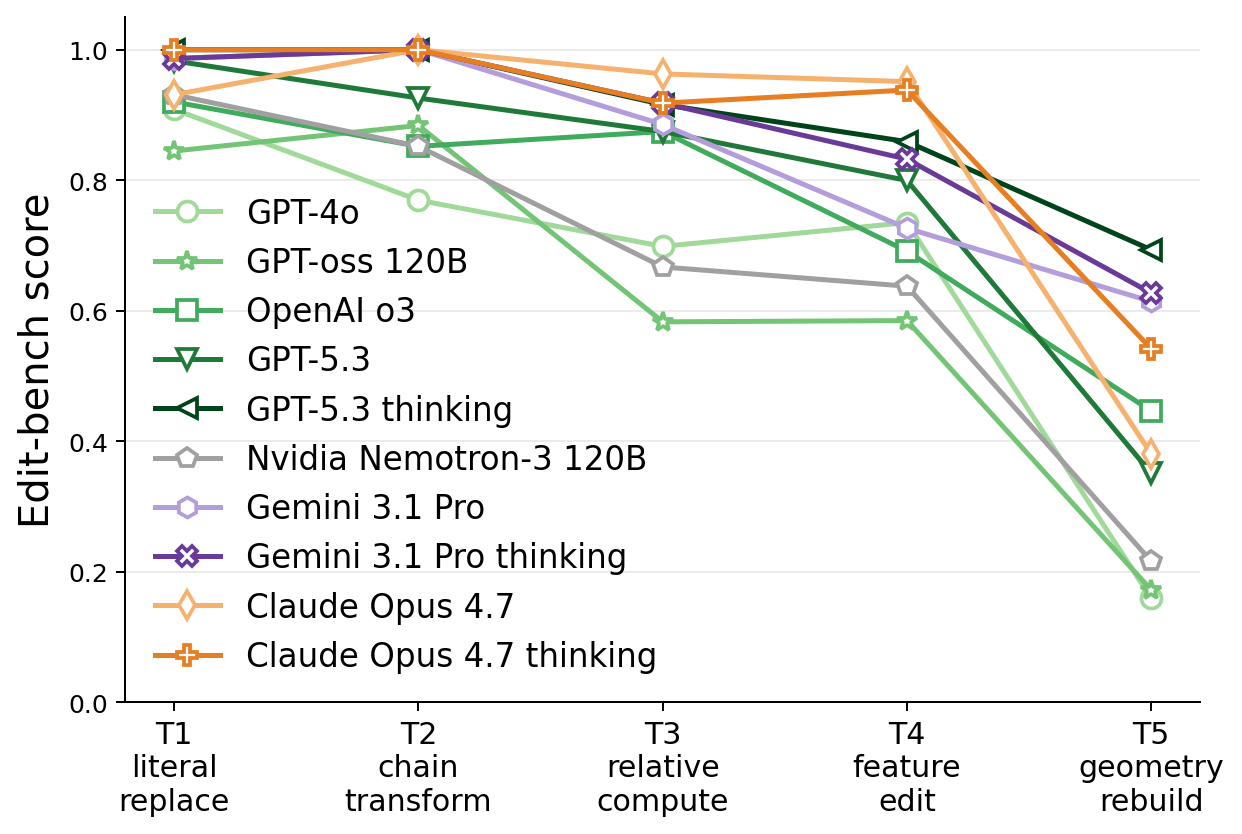
\includegraphics[width=\linewidth]{figures/fig_5.png}   \captionof{figure}{\textbf{BenchCAD-Edit by task type.}}
    \label{fig:edit_task}
  \end{minipage}\hfill                                        \begin{minipage}{0.4\linewidth}                                 \centering                                                    \captionof{table}{\textbf{BenchCAD-Edit Accuracy.}}
    \label{tab:edit_leaderboard}                                \small
\setlength{\tabcolsep}{3pt}
\begin{tabular}{@{}lccc@{}}
\toprule
\textbf{Model}& \textbf{Thinking} & \textbf{Acc.} \\
\midrule
GPT-5.3            & \cmark & \textbf{0.865} \\
Claude Opus 4.7    & \cmark & 0.853 \\
Gemini 3.1 Pro     & \cmark & 0.837 \\
Claude Opus 4.7    & --     & 0.811 \\
Gemini 3.1 Pro     & --     & 0.795 \\
GPT-5.3            & --     & 0.740 \\
OpenAI o3          & \cmark & 0.708 \\
GPT-4o             & --     & 0.615 \\
Nemotron-3 120B    & --     & 0.608 \\
GPT-oss 120B       & --     & 0.561 \\
Baseline (no change) & --     & 0.000 \\
\bottomrule
\end{tabular}
  \end{minipage}
\end{figure} 

\paragraph{\textsc{Code Edit}.} 
\paragraph{Code editing.}
Table~\ref{tab:edit_leaderboard} reports the BenchCAD-Edit leaderboard using mean-normalized improvement as the headline metric, which discounts the varying difficulty of each edit pair. Overall scores show a clear gap between model families, but the per-type breakdown in Fig.~\ref{fig:edit_task} reveals a more diagnostic pattern: simple API-level edits are nearly solved by modern models, while compositional edits remain difficult. The error analysis below ties each regime to specific failure modes; per-model F-code distributions, the full L1--L4 attribution, and the image-conditioned variant are deferred to Appendix~\ref{app:edit_protocol}.


\subsection{Error Analysis}
\label{sec:results_failure_analysis}
\label{sec:exp_failure_analysis}

\begin{wrapfigure}{r}{0.38\linewidth}
  \vspace{-\baselineskip}
  \centering
  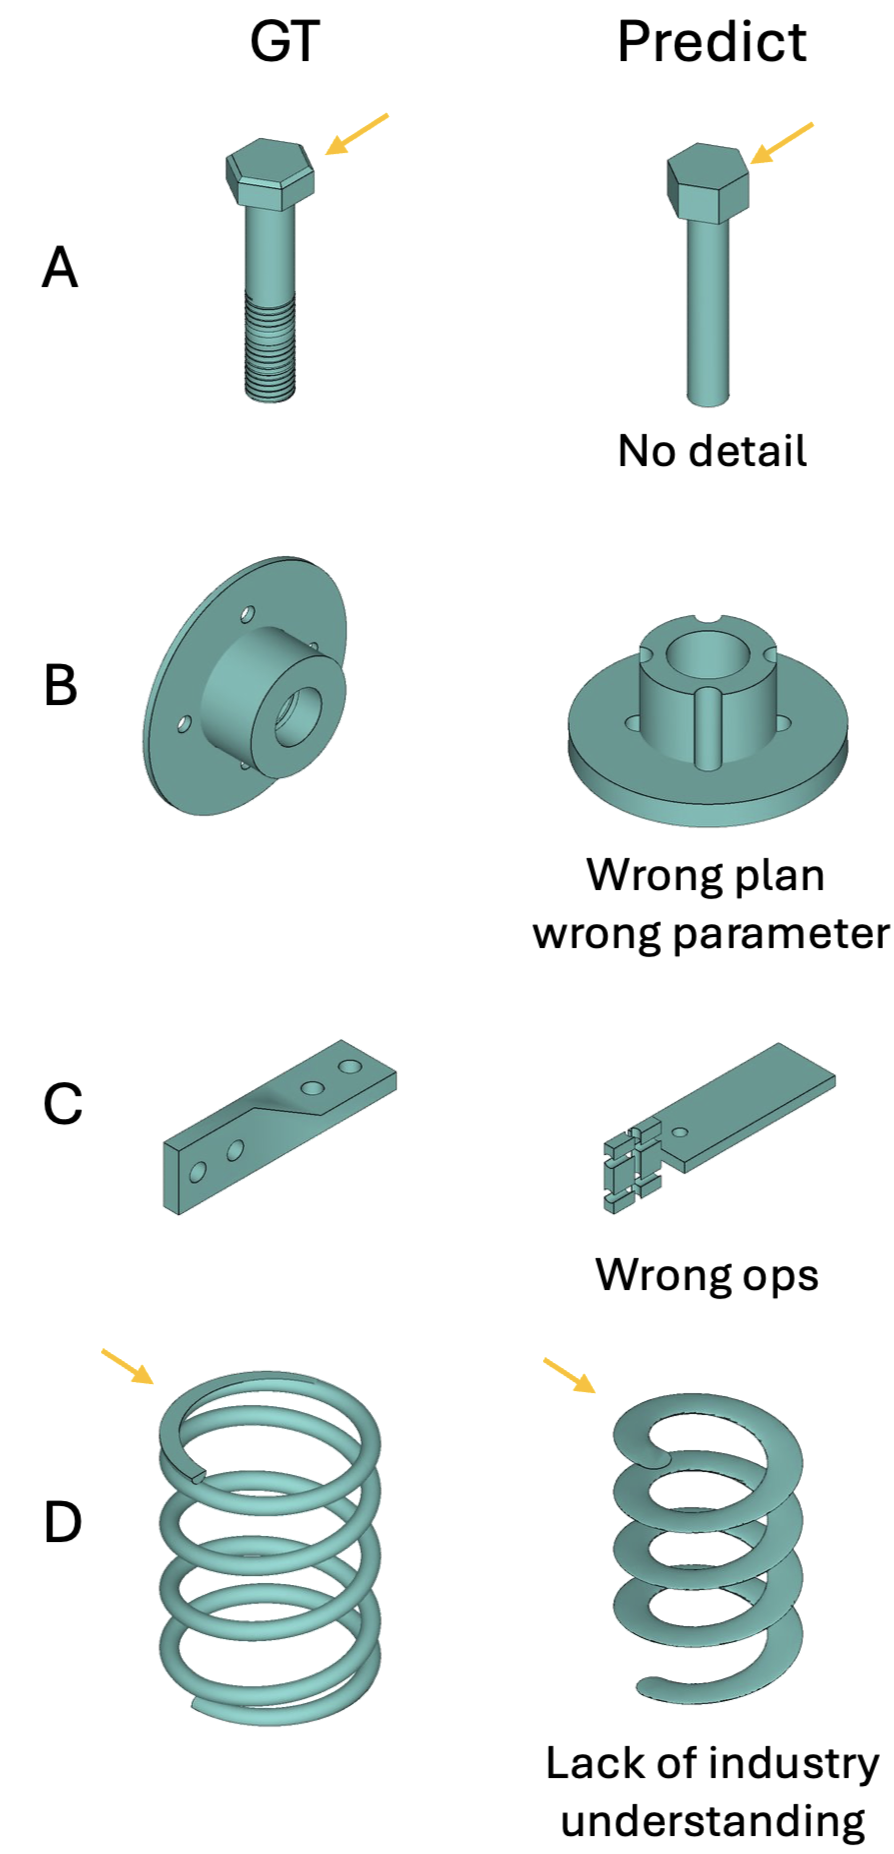
\includegraphics[width=\linewidth]{figures/fig_err_analysis_code_gen.png}
  \caption{\textbf{Examples of failures in codegen.} Zoom-in for more details.}
  \label{fig:err_analysis_codegen}
  \vspace{-0.5\baselineskip}
\end{wrapfigure}

Across tasks, we find that many failures share common causes. Most can be attributed to deficiencies in four core capabilities.


\textbf{Holistic Spatial Recognition}
Visual recognition failures occurs: detailed feature counting and spatial grounding. 
% For instance, 4 out of 8 models fail to identify the keyway adjacent to the central hole in a gear, as the two features are visually blended together in the rendered view.

A hex-head bolt (Figure~\ref{fig:err_analysis_codegen}A) illustrates a fine-detail failure. 
GPT-5.3 recovers the overall bolt body, but omits the threaded shank and chamfered head details. 
The generated part is therefore visually similar at a coarse level but misses small, human-obvious CAD features. 
Consistently, GPT-5.3-chat fails to identify the number of chamfer operations in the corresponding vision QA ($L_1$) on chamfer number. 
Interestingly, though GPT-5.3-thinking answers the chamfer-count question correctly, yet still fails to realize the detail in executable code, suggesting a gap between recognizing a local feature and synthesizing it constructively.

A bearing retainer cap (Figure~\ref{fig:err_analysis_codegen}B) exposes a global spatial-frame failure. 
The model captures several detailed features, but fails to infer the correct extrusion direction: its emitted code extrudes from the XY plane rather than the natural XZ plane. 
This failure is partially diagnosed by the substantially higher 24-axis rotation-invariant IoU compared with the single-axis IoU, indicating that the geometry is partly correct but placed in the wrong spatial frame (\S\ref{app:iou}). 
The same example also reveals parametric-abstraction failures across multiple features.

\textbf{Operation understanding.} A twisted bracket (Figure~\ref{fig:err_analysis_codegen}C) is generated as two mutually perpendicular brackets without twisted connection; the requisite twist-extrusion is absent from the emitted program entirely. 
The model recognizes the holistic spatial (L1) but fails to map the visible torsion to the corresponding CAD operation, exposing an Op Vocabulary Gap (\S\ref{app:op_gap_full}) at the operation-understanding layer.

\textbf{Industrial Parametric abstraction.}
A standardized DIN~2095 coil spring (Figure~\ref{fig:err_analysis_codegen}D) exposes a parametric-abstraction failure. 
The standard requires closed and ground ends: the coil pitch is locally reduced near both terminals, causing the end turns to flatten into planar bearing surfaces. 
The model recognizes the spring and the coil pitch is not a circle, and emits a helical sweep, but collapses this end-specific pitch variation into a uniform helix with an incorrect cross-section.
It therefore captures the coarse family and operation (L1 \& L2) while missing the standard-driven parameterization that an engineer would explicitly encode. 
This failure highlights why BenchCAD anchors its families to engineering standards: the benchmark tests not only whether models can name a part or invoke the right CAD operation, but whether they can recover the structured design rules underlying real parametric CAD.

These cases illustrate how the layered framework converts \textsc{Vision2Code} failures from a single opaque ``wrong code'' category into level-attributable diagnostics: a model can succeed at $L_1$ yet fail at $L_2$ (the bracket), or succeed at $L_1$ and $L_2$ yet fail at $L_3$ (the spring). Without per-level attribution these distinctions collapse into a single low IoU score, and the corresponding training signal --- which level to strengthen --- is lost.

% \textbf{Visual and Code
% Recognition.} Visual recognition failures happen along three axes: detailed feature counting, CAD feature recognition, and spatial grounding. QA asks whether a gear has a keyway, 4/8 models do not find the keyway next to the central cavity.


% We analyze holistic visual recognition failures along three axes: feature counting, CAD feature recognition, and spatial grounding. Models often recognize the presence of repeated structures but fail to count them accurately, especially when they are small, occluded, or densely arranged. They also confuse CAD feature types, such as slots versus holes or protrusions versus cutouts, indicating that coarse silhouette recognition does not imply constructive-geometry understanding. Spatial errors, including misunderstanding the construction plane and rotation axis, as well as incorrect alignment or symmetry judgments, further suggest weak 3D grounding. 



%\textbf{Industrial Parametric Abstraction.} 

%\textbf{Spatial/Code Reasoning.}


%\paragraph{Edit failure-mode breakdown.} A failure-code breakdown (E001--E004 defined in Table~\ref{tab:error_codes}; per-model distribution in Fig.~\ref{fig:edit_error_pies}) shows the dominant failure shifts with model class: \texttt{gpt-4o} and \texttt{gpt-oss-120b} are bottlenecked by \emph{wrong\_operation} (real API, wrong selector or argument); reasoning-tier models trade hallucinations for \emph{no\_op} edits in which the agent rewrites the original byte-for-byte.

%\paragraph{Family Cliff.} Table~\ref{tab:family_cliff} stratifies \texttt{img2cq} pass rate by family difficulty tier. The strongest model collapses by 48\,pt from easy (68\%) to hard (20\%), exhibiting a \textbf{Family Cliff}: hard-tier families exercise advanced operations (helical sweeps, twist-extrusion, lofted Booleans) scarcely present in any prior CAD training corpus, and enforce parametric constraints (gear module--tooth--pitch consistency, spring free-length--turn-count coupling) no model evaluated reliably preserves.

\subsection{Training Findings}
\label{sec:results_training}
\hc{it's a bit unclear why this paragraph is here.}
Our Qwen3-VL-2B trained on BenchCAD achieves SOTA on the in-distribution code-generation benchmark (CodeGen 0.723). When 10 mechanical families are held out, IID-only SFT + RL still transfers non-trivially to the OOD families, indicating that BenchCAD provides useful inductive signal for unseen mechanical structures. Nonetheless, a substantial IID/OOD gap persists, showing that generalization to unseen mechanical families remains an open problem.

\begin{figure*}[t]
  \centering
  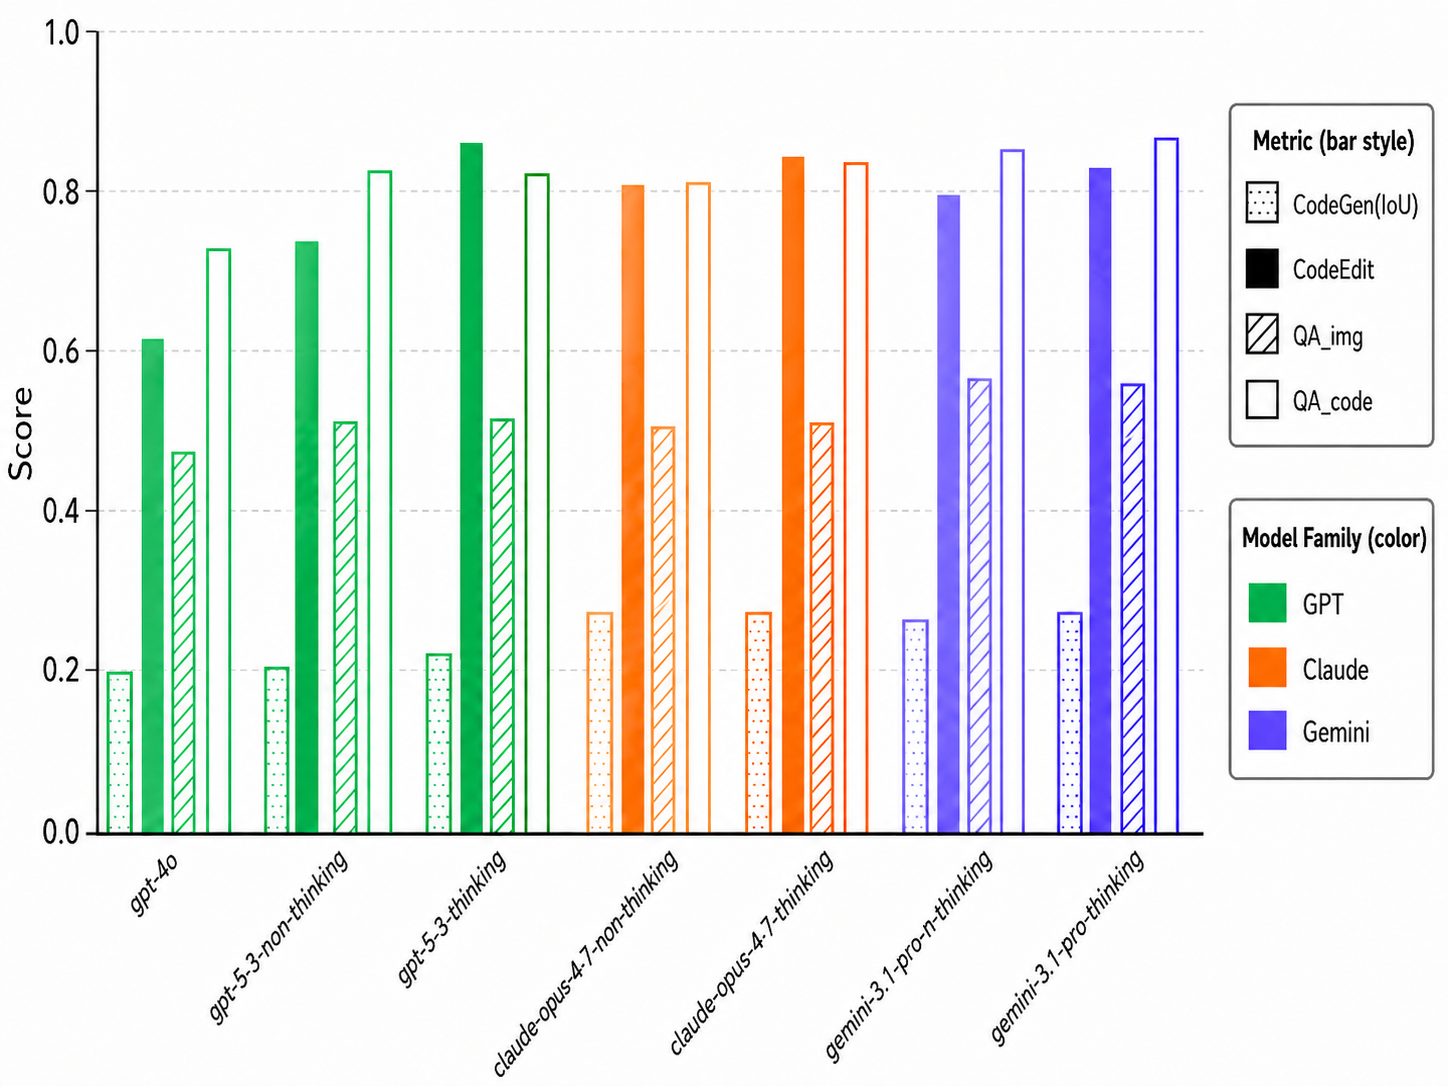
\includegraphics[width=0.65\linewidth]{figures/fig_3.png}
  \caption{\textbf{Per-model performance across the four BenchCAD task categories}
  (frontier proprietary subset; open-source baselines are reported in Table~\ref{tab:main_eval_qa_img}). 
  Bar style encodes task, color encodes model family, and within-family variants distinguish thinking from non-thinking models. 
  Two patterns motivate our subsequent diagnostics: (i) QA-img consistently underperforms QA-code, highlighting the difficulty of holistic spatial recognition from visual evidence; and (ii) CodeEdit trails CodeGen across all models, indicating that instruction-guided modification of existing CAD programs remains harder than greenfield generation.} 
  \label{fig:overall_perform}
\end{figure*}

\section{Conclusion}
\label{sec:conclusion}

BenchCAD is a unified, capability-decomposed evaluation framework for large-model CAD reasoning, anchored in industrial-standard part families and operation-rich CadQuery code.
Across 10+ frontier models, the benchmark reveals three systematic diagnostic phenomena --- the \emph{Vision Bottleneck} ($\sim$15--20\,pt code--image QA gap), \emph{Edit Leakage} ($\sim$64\% of nominally successful edits silently corrupt unrelated features), and the \emph{Op Vocabulary Gap} (matched-compute SFT on sketch+extrude data alone yields zero recall on essential operations).
Together, these findings map both the current state of frontier capability and the focused improvements needed to reach industry-grade CAD generation.
Extended discussion, limitations, and the open BenchCAD-trained reference baseline are deferred to Appendix~\ref{app:discussion}, \ref{app:limitations}, and \ref{app:baseline}.
Dataset, evaluation harness, and Croissant 1.0 metadata are released under CC-BY-4.0 at \texttt{huggingface.co/BenchCAD}.


\begin{ack}
\textcolor{red}{[Anonymised for submission. Restore acknowledgments and funding disclosure for camera-ready.]}
\end{ack}

\bibliographystyle{plainnat}
\bibliography{refs}

% --- appendix ---
\appendix

\section{Limitations}
\label{app:limitations}

\paragraph{Standard-parametric coverage is not full industrial CAD.} BenchCAD parts are generated from expert-authored standard-parametric families, not extracted from real engineering repositories.
We mitigate this by (i) anchoring 49\% of families to published ISO/DIN/EN/ASME/IEC specification tables and (ii) including verified Fusion360 Gallery and DeepCAD subsets for OOD comparison, but our parts do not capture the full diversity of proprietary industrial design (e.g.\ hand-drawn manufacturing tolerances, undocumented design intent, assembly information).

\paragraph{Standard-anchored does not mean standard-compliant.} A family declared as \texttt{standard = "ISO 23509"} samples within ISO parameter ranges and enforces inter-parameter relations from the standard, but does not validate against the full set of manufacturing tolerances or material specifications mandated by that standard.

\paragraph{Industrial Common Sense Gap measurement.} Our non-target preservation metric uses voxel IoU on the spatial complement of the targeted feature; this captures most leakage modes but can miss small parametric shifts whose voxel footprint is subthreshold.
\S\ref{app:edit_protocol} discusses the protocol, including a complementary code-AST diff metric we report alongside.

\section{Extended Related Work: CAD Code-Generation and Editing Benchmarks}
\label{app:related_extended}

\paragraph{Code generation.}
DeepCAD~\citep{Wu2021} introduces a 178K-model corpus of Onshape parts encoded as discrete operation tokens; Text2CAD~\citep{Khan2024} extends DeepCAD with 660K natural-language annotations across four abstraction levels. CAD-Coder~\citep{Guan2025} reformulates the same data as CadQuery Python source and applies SFT$+$GRPO with chain-of-thought and Chamfer reward (mean CD $6.54{\times}10^{-3}$ on Text2CAD). The CAD-Recode~\citep{Rukhovich2025}/cadrille~\citep{Kolodiazhnyi2026}/CADEvolve~\citep{Elistratov2026} lineage shares a Qwen2-VL-2B backbone: CAD-Recode fine-tunes on 1M sketch-and-extrude scripts (DeepCAD IoU 92.0); cadrille adds multi-modal inputs and Dr.CPPO online RL with piecewise IoU reward (DeepCAD IoU 92.2, Fusion360 IoU 84.6, 0.0\% invalidity); CADEvolve expands the corpus to $\sim$1.3M scripts via an LLM-driven evolutionary loop covering extrude/revolve/loft/sweep/fillet/chamfer/shell/Boolean/patterns (DeepCAD IoU 92.6) --- broadening the operation distribution but still without helical sweeps or parametric involute-gear construction. The CADEvolve Hugging Face release contains only sentence embeddings (\texttt{.npy}), not the source code, so its full operation surface is not directly auditable; the public GitHub repo ships only $46$ hand-written seed programs.

\paragraph{Editing.}
CADPrompt~\citep{Alrashedy2025} introduces 200 NL$\to$CadQuery prompts scored via point-cloud distance and bounding-box IoU after ICP alignment --- two orders of magnitude smaller than BenchCAD-Edit (17{,}900), without family taxonomy or difficulty stratification, and with potential scale leakage from absolute mm cues and axis-aligned IoU. CAD-Editor~\citep{CADEditor2025} trains a locate-then-infill editor entirely on synthetic edits, but releases no held-out human-verified edit benchmark. CADialogue~\citep{CADialogue2025} evaluates ten edit tasks in a conversational CAD interface, but does not release the eval set. HistCAD~\citep{Dong2026} evaluates constraint preservation under FreeCAD edits, but at the sketch-constraint rather than executable-program level. BenchCAD-Edit is, to our knowledge, the first public CAD editing benchmark with execution-verified before/after CadQuery pairs, preservation-aware metrics, and balanced cross-family edit-category coverage.

\section{Full Comparison Against Prior CAD Code-Generation Work}
\label{app:cmp_prior}

Table~\ref{tab:cmp_prior} provides the full per-axis comparison referenced in \S\ref{sec:related}, including all evaluation-side properties (\#Industrial families, \#Std codes, \#Distinct CQ ops, Adv ops, Edit / QA tasks, \#Eval models) across DeepCAD, Fusion360 Gallery, Text2CAD, CADPrompt, CAD-Coder, CAD-Recode, cadrille, and CADEvolve.

\begin{table*}[t]
\centering
\small
\setlength{\tabcolsep}{5pt}
\caption{\textbf{BenchCAD versus prior CAD code-generation work.} BenchCAD is a \emph{unified, capability-decomposed evaluation framework} for large-model CAD reasoning, distinct in purpose from the CadQuery-VLM lineage (CAD-Recode, cadrille, CADEvolve) which releases training corpora alongside small fine-tuned models (Qwen 1.5B--2B) saturating $\sim$92\% IoU on legacy sketch+extrude splits. \textbf{Type:} \emph{C+M} = corpus+model, \emph{D} = dataset, \emph{B} = benchmark. \textbf{\#Fam.} = named industrial part families with explicit functional identity. \textbf{\#Std} = distinct ISO/DIN/EN/ASME/IEC specification codes. \textbf{\#Ops} = distinct CadQuery API methods exercised in the released corpus (static analysis of every released \texttt{.py}; see Appendix~\ref{app:ops}). \textbf{Adv} = all four advanced operation families (helix, loft/sweep, twist-extrude, parametric involute-gear) exercised. $\checkmark$ = supported, p.\ = partial, -- = absent.}
\label{tab:cmp_prior}
\begin{tabular}{lccrrrrccc}
\toprule
Benchmark & Yr & Type & \#Sam. & \#Fam. & \#Std & \#Ops & Adv & Edit & QA \\
\midrule
DeepCAD~\citep{Wu2021}                   & '21 & C+M & 178K  & -- & 0  & 4   & --   & --   & --   \\
Fusion360 G.~\citep{Willis2021fusion}    & '21 & D   & 8K    & -- & 0  & 6   & --   & --   & --   \\
Text2CAD~\citep{Khan2024}                & '24 & C+M & 170K  & -- & 0  & 17  & --   & --   & --   \\
CADPrompt~\citep{Alrashedy2025}          & '25 & B   & 200   & -- & 0  & --  & p.\  & --   & --   \\
CAD-Coder~\citep{Guan2025}               & '25 & C+M & 110K  & -- & 0  & 4   & --   & p.\  & --   \\
CAD-Recode~\citep{Rukhovich2025}         & '25 & C+M & 1M+7K & -- & 0  & 18  & --   & p.\  & seq.\\
cadrille~\citep{Kolodiazhnyi2026}        & '26 & C+M & 1M+7K & -- & 0  & 18  & --   & --   & --   \\
CADEvolve~\citep{Elistratov2026}         & '26 & C+M & 2.7M  & -- & 0  & 25  & p.\  & --   & --   \\
\midrule
\textbf{BenchCAD (ours)} & \textbf{'26} & \textbf{D+B} & \textbf{17{,}900} & \textbf{106} & \textbf{43} & \textbf{49} & $\checkmark$ & $\checkmark$ & $\checkmark$ \\
\bottomrule
\end{tabular}
\end{table*}

\section{Standard Codes Covered}
\label{app:standards}
Table~\ref{tab:standards} reports the standards grounding of BenchCAD. 
Nearly half of all families, 52/106 (49\%), are tied to ISO, DIN, EN, ASME, or IEC specification tables, so their dimensions are sampled from real engineering ranges rather than arbitrary shapes. 
The remaining 54 custom families cover bespoke industrial parts without a formal standard, while still using analogous proportional design rules.

\begin{table}[t]
\centering
\small
\caption{\textbf{Standard-anchored families.} 55\% of BenchCAD families bind their parameters to ISO/DIN/EN/ASME/IEC specification tables, sampling at values drawn from real engineering ranges rather than arbitrary geometry. The bottom row lists the 47 custom families covering bespoke industrial parts (twisted brackets, lobed knobs) governed by analogous proportional rules without formal standards.}
\label{tab:standards}
\begin{tabular}{llr}
\toprule
Standard & Codes covered (sample) & \#Fam. \\
\midrule
ISO   & 22, 113, 272, 1234, 2339, 2936, 10828, 23509, \ldots & 22 \\
DIN   & 338, 471/472, 580, 5480, 2095, 8187, 71412, \ldots    & 28 \\
EN    & 10034, 10056, 10219, 10279                            & 4  \\
ASME  & B1.20.1, B16.5, B16.9                                 & 3  \\
IEC   & 60072-1, 60086                                        & 2  \\
\midrule
\textbf{Total standard-anchored}   &                              & \textbf{59 (55\%)} \\
Custom (no formal standard)        &                              & 47 \\
\bottomrule
\end{tabular}
\end{table}


\section{Dataset Generation Details}
\label{app:datagen}

\paragraph{Subfamilies.} A family may further branch into one or more \emph{subfamilies} that capture mating, assembly, or construction variants of the same part type --- for instance, a threaded-fastener family may split into male (\texttt{bolt}) and female (\texttt{nut}) subfamilies that share the same thread/pitch parameter table but differ in build chain; a retaining-ring family may split into internal (groove inside a bore) and external (groove on a shaft) variants; a thread family may split into single- and multi-start helices. Subfamilies reuse their parent family's parameter schema and standard-table anchoring, but specify their own deterministic builder. They are sampled and rendered independently, so a single named family in the per-family analysis can contribute several subfamily$\times$tier buckets to the verified release.

\paragraph{Difficulty tiers.} Each (sub)family exposes three tiers --- \emph{easy} / \emph{medium} / \emph{hard} --- defined by parameter complexity. Easy uses default parameter ranges with optional features disabled (e.g., a coil spring with constant pitch and no end treatment). Medium expands parameter ranges and enables a subset of optional features. Hard activates all optional features and uses extreme but still standard-compliant parameter ranges (e.g., variable pitch with closed-and-ground spring ends), exercising the more advanced construction operations of the family. Sampling is balanced approximately uniformly across tiers within each (sub)family.

\paragraph{Sandbox failure-mode taxonomy.} Each generated CadQuery program is executed in a sandbox subprocess; records hitting any of the following are quarantined and excluded from the release: (i) \emph{parse / import error} --- the program fails Python parsing or CadQuery API resolution; (ii) \emph{runtime exception} --- a CadQuery call raises (e.g., on a non-positive radius or an empty selector); (iii) \emph{timeout} --- execution exceeds a 30\,s wall-clock budget, typically caused by pathological boolean or sweep construction; (iv) \emph{degenerate volume} --- the resulting solid has $\leq 10^{-6}$\,mm$^3$ volume or an inverted (negative-determinant) transformation chain. Programs surviving all four checks are rendered into multi-view images and routed past a domain expert for visual sign-off; only records passing every stage enter the release.

\section{Full Per-Model Per-Task Results}
\label{app:full_results}

Table~\ref{tab:dataset} reports the dataset composition; Table~\ref{tab:capability} maps each task to its sub-capability subset; Tables~\ref{tab:main_eval_qa_img} and~\ref{tab:main_eval_qa_code} report the per-model QA leaderboard (Vision QA / Code QA); Table~\ref{tab:family_cliff} stratifies \texttt{img2cq} by family difficulty. The unified Vision2Code leaderboard (Table~\ref{tab:codegen_unified}) is in the main body.

\begin{table}[t]
\centering
\small
\caption{\textbf{BenchCAD dataset composition.} Three released datasets: the verified CadQuery code core (17{,}900 parts spanning 106 families, each with parametric source, executable STEP, four canonical-view renders, parameter JSON, and op list), the paired QA bank (2{,}400 questions evaluated under both visual and code conditioning), and the Edit subset (748 before/after pairs).}
\label{tab:dataset}
\begin{tabular}{lrrl}
\toprule
Dataset & \#Records & \#Families & GT artefacts \\
\midrule
BenchCAD                     & 17{,}900             & 106 & code $\cdot$ STEP $\cdot$ 4 views $\cdot$ params $\cdot$ ops \\
BenchCAD-QA (paired img/code)& 2{,}400 $\times 2$   & 106 & question $+$ gold answer \\
BenchCAD-Edit                & 748                  & 106 & before/after $+$ NL instruction \\
\bottomrule
\end{tabular}
\end{table}


\begin{table}[t]
\centering
\small
\caption{\textbf{Capability decomposition.} BenchCAD's five tasks isolate the three sub-capabilities along the image$\to$code causal chain: $C_1$ visual + 3D reconstruction, $C_2$ geometric$\to$parametric abstraction, and $C_3$ parametric$\to$code synthesis. Score differences across paired tasks (e.g.\ \texttt{qa\_img}$-$\texttt{qa\_code}) directly diagnose which capability is the bottleneck. ``part.'' indicates partial coverage (the original code constrains, but does not eliminate, the corresponding sub-capability).}
\label{tab:capability}
\begin{tabular}{llccc}
\toprule
Task & Input $\to$ Output & $C_1$ vision & $C_2$ param. & $C_3$ code \\
\midrule
\texttt{img2cq}    & 4 views $\to$ code              & \cmark & \cmark & \cmark \\
\texttt{qa\_img}   & 4 views $+$ Q $\to$ number      & \cmark & \cmark & --     \\
\texttt{qa\_code}  & code $+$ Q $\to$ number         & --     & \cmark & --     \\
\texttt{edit\_img} & views $+$ code $+$ instr $\to$ code  & \cmark & part.  & \cmark \\
\texttt{edit\_code}& code $+$ instr $\to$ code       & --     & part.  & \cmark \\
\bottomrule
\end{tabular}
\end{table}


\begin{table*}[t]
\centering
\small
\setlength{\tabcolsep}{5pt}
\renewcommand{\arraystretch}{1.15}
\caption{\textbf{Main evaluation on BenchCAD-QA (\texttt{qa\_code} modality), by capability axis.} Per-model accuracy on the code-conditioned QA bank across the same four capability axes as Table~\ref{tab:main_eval_qa_img}. The two tables share questions and capability-axis definitions; only the conditioning modality differs (rendered images vs.\ source CadQuery). Score differences across the matched pair isolate the cost of replacing direct code access with visual recognition --- the \textbf{Holistic Spatial and Detailing Deficit}.}
\label{tab:main_eval_qa_code}
\begin{tabular}{l c c c c c}
\toprule
Model
 & \shortstack{Cadquery Code\\Recognition $\uparrow$ }
 & \shortstack{CAD Operation\\Understanding $\uparrow$ }
 & \shortstack{Industrial Parametric\\Abstraction $\uparrow$ }
 & \shortstack{Spatial\\Reasoning $\uparrow$ }
 & \shortstack{Total\\score $\uparrow$ } \\
\midrule
opus-4.7         & 0.868 & 0.800 & 0.793 & 0.595 & 0.801 \\
opus-4.7-thinking            & 0.891 & 0.781 & 0.851 & 0.632 & 0.829 \\
gemini-3.1-pro  & \textbf{0.914} & 0.782 & 0.867 & 0.537 & 0.836 \\
gemini-3.1-pro-thinking     & 0.907 & 0.783 & \textbf{0.876} & 0.537 & \textbf{0.838} \\
gpt-4o                              & 0.865 & 0.593 & 0.732 & 0.688 & 0.726 \\
gpt-5.3-chat-latest                 & 0.879 & \textbf{0.805} & 0.815 & 0.731 & 0.823 \\
gpt-5.3-thinking                    & 0.885 & 0.802 & 0.811 & 0.730 & 0.821 \\
moonshot-v1-128k-v     & 0.842    & 0.551    & 0.692    & \textbf{0.792}    & 0.700 \\                                                                       
  moonshot-v1-8k-v       & 0.772    & 0.603    & 0.555    & 0.536    & 0.620 \\               
openai-o3                & 0.804    & 0.701    & 0.689    & 0.492    & 0.708 \\                                                                
  google-gemma-4-31b-it    & 0.791    & 0.674    & 0.606    & 0.528    & 0.664 \\                                                                
  openai-gpt-oss-120b      & 0.790    & 0.732    & 0.656    & 0.379    & 0.689 \\
  nvidia-nemotron-3-120b   & 0.771    & 0.660    & 0.661    & 0.293    & 0.671 \\       
\midrule
\textit{blank code (baseline)}     & 0.040    & 0.257    & 0.290    & 0.420    & 0.223    \\
\bottomrule
\end{tabular}
\end{table*}


\begin{table}[t]
\centering
\small
\setlength{\tabcolsep}{6pt}
\renewcommand{\arraystretch}{1.05}
\caption{\textbf{Vision2Code unified leaderboard.} Specialist CAD lineage (cadrille / CADEvolve), frontier MLLMs, and our open Qwen3-VL-2B trained baseline. All BenchCAD scores on BenchCAD-Lite. \emph{(\,$\dagger$\,)} Ours-SFT-IID is evaluated on the IID split (all 106 families seen at train time); all other rows are OOD on BenchCAD by construction (specialist lineage and frontier MLLMs never saw BenchCAD; ours-SFT-OOD / +RL hold out 10 mech.-transmission families). Essential-op recall is the fraction of ground-truth essential operations (helix / sweep / loft / twist-extrude / parametric involute-gear) recovered by the prediction.}
\label{tab:codegen_unified}
\begin{tabular}{@{}lcccl@{}}
\toprule
Model                                                  & DeepCAD IoU      & BenchCAD IoU            & Ess.\ op recall  & Notes \\
\midrule
\multicolumn{5}{l}{\emph{Specialist CAD lineage ($\sim$2B, OOD on BenchCAD)}} \\
cadrille-RL~\citep{Kolodiazhnyi2026}                   & 0.919            & 0.273                   & --               & sketch+ext, 1M \\
CADEvolve~\citep{Elistratov2026}                       & 0.923            & 0.039                   & --               & extended, 2.7M \\
\midrule
\multicolumn{5}{l}{\emph{Frontier MLLMs (BenchCAD-Lite, by def.\ OOD)}} \\
gpt-4o                                                 & --               & 0.188                   & 0.468            & \\
gpt-5.3 (thinking)                                     & --               & 0.207                   & 0.455            & \\
claude-opus-4.7 (thinking)                             & --               & 0.267                   & 0.471            & \\
gemini-3.1-pro (thinking)                              & --               & \textbf{0.279}          & \textbf{0.567}   & strongest frontier \\
\midrule
\multicolumn{5}{l}{\emph{Ours --- Qwen3-VL-2B, 9 GPU-h on $8{\times}$A800-80GB}} \\
SFT (IID, 106 fam.\ seen)$^{\dagger}$                  & --               & \textbf{0.650}          & \textbf{0.950}   & dataset learnable on 2B \\
SFT (OOD, 10 fam.\ held out)                           & --               & 0.180                   & 0.200            & generalisation gap \\
\quad $+$ RL ($r{=}0.2\,\mathrm{ess}{+}0.8\,\mathrm{IoU}$) & --             & 0.350                   & 0.450            & RL partial recovery \\
\bottomrule
\end{tabular}
\end{table}


\begin{table}[t]
\centering
\small
\caption{\textbf{The Family Cliff.} \texttt{img2cq} pass rate (\%) split by family difficulty tier. Even the strongest reasoning model collapses on the hard tier, exhibiting a $>$45-point gap from easy. The 26 hard-tier families exercise advanced operations (helical sweeps, twist-extrusion, lofted Booleans) and parametric constraints (gear module--tooth--pitch consistency, spring free-length--turn-count coupling) that no evaluated model reliably preserves. \textcolor{red}{Numbers are placeholders.}}
\label{tab:family_cliff}
\begin{tabular}{lrrrr}
\toprule
Model & Easy (40 fam.) & Medium (40 fam.) & Hard (26 fam.) & $\Delta$ E$-$H \\
\midrule
GPT-5.3 (think)          & 68 & 42 & \textbf{20} & \textbf{48} \\
Claude Opus 4.7 (think)& 65 & 40 & 19 & 46 \\
GPT-4o                 & 52 & 28 & 9  & 43 \\
Qwen2.5-VL-72B         & 38 & 18 & 5  & 33 \\
InternVL3-1B           & 15 & 4  & 1  & 14 \\
\bottomrule
\end{tabular}
\end{table}


\section{CAD Operational Blindspot: Per-Operation Recall}
\label{app:op_gap_full}
Table~\ref{tab:op_recall} reports the recall of operations.

\begin{table}[t]
    \centering
    \small
    \setlength{\tabcolsep}{4pt}
    \caption{\textbf{TODO Per-operation recall on Vision2Code} with paired comparison of gpt-5.3 (chat-latest) vs gpt-5.3-thinking.              
    Thinking-mode degrades both macro recall (advanced: 25.2 → 22.8, all: 35.1 → 32.3) and execution rate (69.5 → 
    67.5), against the common expectation that inference-time reasoning monotonically helps. Looking inside the per-op 
    deltas reveals a structural trade: thinking improves recall on composition-choice and finishing operations that 
    benefit from explicit planning (loft +17.6, polygon +18.2, fillet +12.0, rarray +7.2) but degrades on direct       
    boolean and scaffolding operations (cut −11.9, cutBlind −10.5, workplane −8.9, sweep −7.7, box −7.7, union −5.6). 
    The net effect is a synthesis-execution trade-off
    — the model thinks more about which high-level op
    to call, while writing the surrounding boilerplate
    less reliably.}
    \label{tab:op_recall}
  \begin{tabular}{lrrr}                                             
  \toprule                                                                                 
  Operation & gpt-5.3 & gpt-5.3-thk & $|\text{GT}|$ \\                                                             
  \midrule                                                                                                             
  \multicolumn{4}{l}{\emph{Basic ops (shared with prior corpora: cad-recode / text2cad)}} \\                           
  \texttt{extrude}              & 83.3          & \textbf{84.4} & 90  \\                                               
  \texttt{cut}                  & \textbf{44.1} & 32.2          & 59  \\                                               
  \texttt{union}                & \textbf{65.3} & 59.7          & 72  \\                                               
  \texttt{circle}               & \textbf{78.7} & 77.3          & 75  \\                                               
  \texttt{cylinder}             & 4.5           & \textbf{7.6}  & 66  \\                                               
  \texttt{box}                  & \textbf{42.3} & 34.6          & 78  \\                                               
  \texttt{rect}                 & 63.0          & \textbf{65.2} & 46  \\                                               
  \texttt{workplane}            & \textbf{86.3} & 77.4          & 124 \\                                               
  \midrule                                                                                                             
  \multicolumn{4}{l}{\emph{Advanced ops (BenchCAD-distinguishing)}} \\                                                 
  \texttt{hole}                 & \textbf{60.2} & 55.4          & 83  \\                                               
  \texttt{chamfer}              & \textbf{8.6}  & 4.3           & 70  \\                                               
  \texttt{cutThruAll}           & \textbf{16.2} & 10.8          & 37  \\                                               
  \texttt{revolve}              & \textbf{14.3} & 10.7          & 28  \\                                               
  \texttt{fillet}               & 0.0           & \textbf{12.0} & 25  \\
  \texttt{cutBlind}             & \textbf{36.8} & 26.3          & 19  \\                                               
  \textbf{\texttt{loft}}        & 5.9           & \textbf{23.5} & 17  \\
  \texttt{threePointArc}        & \textbf{6.2}  & 0.0           & 16  \\                                               
  \texttt{rarray}               & 7.1           & \textbf{14.3} & 14  \\                                               
  \textbf{\texttt{sweep}}       & \textbf{53.8} & 46.2          & 13  \\                                               
  \texttt{polygon}              & 54.5          & \textbf{72.7} & 11  \\                                               
  \texttt{makeHelix}            & 12.5          & 12.5          & 8   \\                                               
  \texttt{slot2D}               & 25.0          & 25.0          & 8   \\                                               
  \texttt{polarArray}           & 20.0          & 20.0          & 5   \\                                               
  \texttt{shell}                & \textbf{25.0} & 0.0           & 4   \\
  \texttt{mirrorY}              & 0.0           & 0.0           & 4   \\                                               
  \texttt{sphere}               & 100.0         & 100.0         & 4   \\
  \texttt{cboreHole}            & 0.0           & 0.0           & 3   \\                                               
  \texttt{radiusArc}            & \textbf{33.3} & 0.0           & 3   \\
  \midrule                                                                                                             
  \textbf{Macro recall} (advanced, 19 ops) & \textbf{25.2\%} & 22.8\% & --- \\
  \textbf{Macro recall} (all, 27 ops)      & \textbf{35.1\%} & 32.3\% & --- \\                                         
  \textbf{Exec rate}                       & \textbf{69.5\%} & 67.5\% & --- \\                                         
  \bottomrule                                                                                                          
  \end{tabular}                                                                                                       
                                     
    % \begin{tabular}{lrrrr}
    % \toprule
    % Operation & baseline & ood & iid & $|\text{GT}|/100$ \\
    % \midrule
    % \multicolumn{5}{l}{\emph{Basic ops (shared with prior corpora: cad-recode / text2cad)}} \\
    % \texttt{extrude}              & 100.0 & 91.7  & 95.8  & 24 \\
    % \texttt{cut}                  & 87.2  & 70.2  & 89.4  & 47 \\
    % \texttt{union}                & 91.7  & 41.7  & 79.2  & 24 \\
    % \texttt{circle}               & 82.8  & 79.3  & 96.6  & 29 \\
    % \texttt{cylinder}             & 5.9   & 88.2  & 94.1  & 17 \\
    % \texttt{box}                  & 2.6   & 84.6  & 92.3  & 39 \\
    % \texttt{rect}                 & 5.0   & 65.0  & 90.0  & 20 \\
    % \texttt{workplane}            & 0.0   & 77.4  & 88.7  & 53 \\
    % \midrule
    % \multicolumn{5}{l}{\emph{Advanced ops (BenchCAD-distinguishing)}} \\
    % \textbf{\texttt{revolve}}     & \textbf{0.0} & \textbf{54.8} & \textbf{93.5} & 31 \\
    % \textbf{\texttt{loft}}        & \textbf{0.0} & \textbf{22.2} & \textbf{77.8} &  9 \\
    % \textbf{\texttt{sweep}}       & \textbf{0.0} & \textbf{25.0} & \textbf{75.0} &  8 \\
    % \textbf{\texttt{sweep+helix}} & \textbf{0.0} & \textbf{100.0}& \textbf{50.0} &  2 \\
    % \textbf{\texttt{twistExtrude}}& \textbf{0.0} & \textbf{100.0}& \textbf{100.0}&  1 \\
    % \texttt{fillet}               & 0.0   & 25.0  & 87.5  &  8 \\
    % \texttt{chamfer}              & 0.0   & 85.3  & 85.3  & 34 \\
    % \texttt{shell}                & 0.0   & 80.0  & 100.0 &  5 \\
    % \texttt{hole}                 & 0.0   & 82.8  & 93.1  & 29 \\
    % \texttt{rarray}               & 0.0   & 77.8  & 100.0 &  9 \\
    % \texttt{polarArray}           & 0.0   & 33.3  & 83.3  &  6 \\
    % \midrule
    % \textbf{Macro recall} (16 ops) & \textbf{17.5\%} & \textbf{59.9\%} & \textbf{84.0\%} & --- \\
    % \textbf{Exec rate}             & 90.0\% & 94.0\% & 99.0\%        & --- \\
    % \bottomrule
    % \end{tabular}
    \end{table}

    

\section{Model Training}
\paragraph{SFT training mixture.}
(1) \textbf{iid}: BenchCAD (all 106 families) + extrusion-heavy data (text2cad, cad-recode);
(2) \textbf{ood}: same recipe, 10 mechanical families held out;
(3) \textbf{baseline}: text2cad + cad-recode only (no BenchCAD).
Mixing 33\% BenchCAD / 67\% HQ for (1)/(2); 100\% HQ for (3). Backbone Qwen3-VL-2B.

\paragraph{OOD holdout selection.}
We hold out 10 CAD families sampled uniformly at random from BenchCAD families that are sufficiently represented and the operations are covered in the iid but not in the baseline.

\paragraph{SFT training setup.}
We fine-tune Qwen3-VL-2B-Instruct under a standard supervised code-generation setup. Inputs consist of one rendered view and a textual instruction, and targets are CadQuery programs.We use AdamW with
learning rate $2{\times}10^{-4}$, cosine decay, $2$k warmup steps, weight decay $0.01$ with bf16 precision.

\paragraph{RL training setup.}
We initialize RL from the matching SFT checkpoint: IID-SFT uses the full BenchCAD training set, whereas OOD-SFT excludes the held-out OOD families. RL is trained with a top-$N$ GRPO-style objective without advantage normalization on a mixed prompt pool from BenchCAD, DeepCAD, and Fusion360; in the OOD setting, the held-out families remain excluded. Rewards combine geometric fidelity with an essential-operation term when available. We use learning rate $2{\times}10^{-5}$, 16 rollouts per prompt, and batch size 128.

\begin{table}[t]
\centering
\small
\setlength{\tabcolsep}{5pt}
\renewcommand{\arraystretch}{1.08}
\caption{\textbf{IID--OOD generalization under SFT and RL.}
We report geometric fidelity, execution rate, essential-operation score, and the final score.}
\label{tab:iid_ood}
\begin{tabular}{@{}llccccc@{}}
\toprule
Checkpoint & Split & IoU$\uparrow$ & Exec.$\uparrow$ & Ess.$\uparrow$ & Score$\uparrow$ \\
\midrule
\multirow{2}{*}{ood-sft (A)}
& IID  & 0.577 & 94.6\% & 0.789 & 0.6064 \\
& OOD  & 0.397 & 89.8\% & 0.305 & 0.3776 \\
\midrule
\multirow{2}{*}{ood-rl (B)}
& IID & 0.757 & 99.1\%  & 0.865 & 0.7467 \\
& OOD  & 0.464 & \textbf{100.0\%} & 0.339 & 0.4604 \\
\midrule
\multirow{2}{*}{iid-sft (C)}
& IID & 0.640 & 87.3\% & 0.857 &  0.6225 \\
& OOD  & \ 0.635 & 96.6\% & 0.983 & 0.6920 \\
\midrule
\multirow{2}{*}{iid-rl (D)}
& IID & 0.753 & 98.9\% & 0.883 & 0.7635 \\
& OOD & \textbf{0.761} & 99.6\% & \textbf{0.989} & \textbf{0.8214} $\star$ \\
\bottomrule
\end{tabular}
\end{table}
\paragraph{Model Generalization.}
Table~\ref{tab:iid_ood} separates IID performance from held-out OOD-family generalization. 
RL substantially improves the OOD-SFT checkpoint on both IID and OOD splits, indicating that geometry-based optimization improves execution and fidelity beyond supervised imitation. 
However, the IID-trained SFT model still achieves the strongest OOD score, suggesting that broad family coverage during training remains the dominant factor for generalizing to unseen mechanical designs.

\begin{figure*}[t]
  \centering
  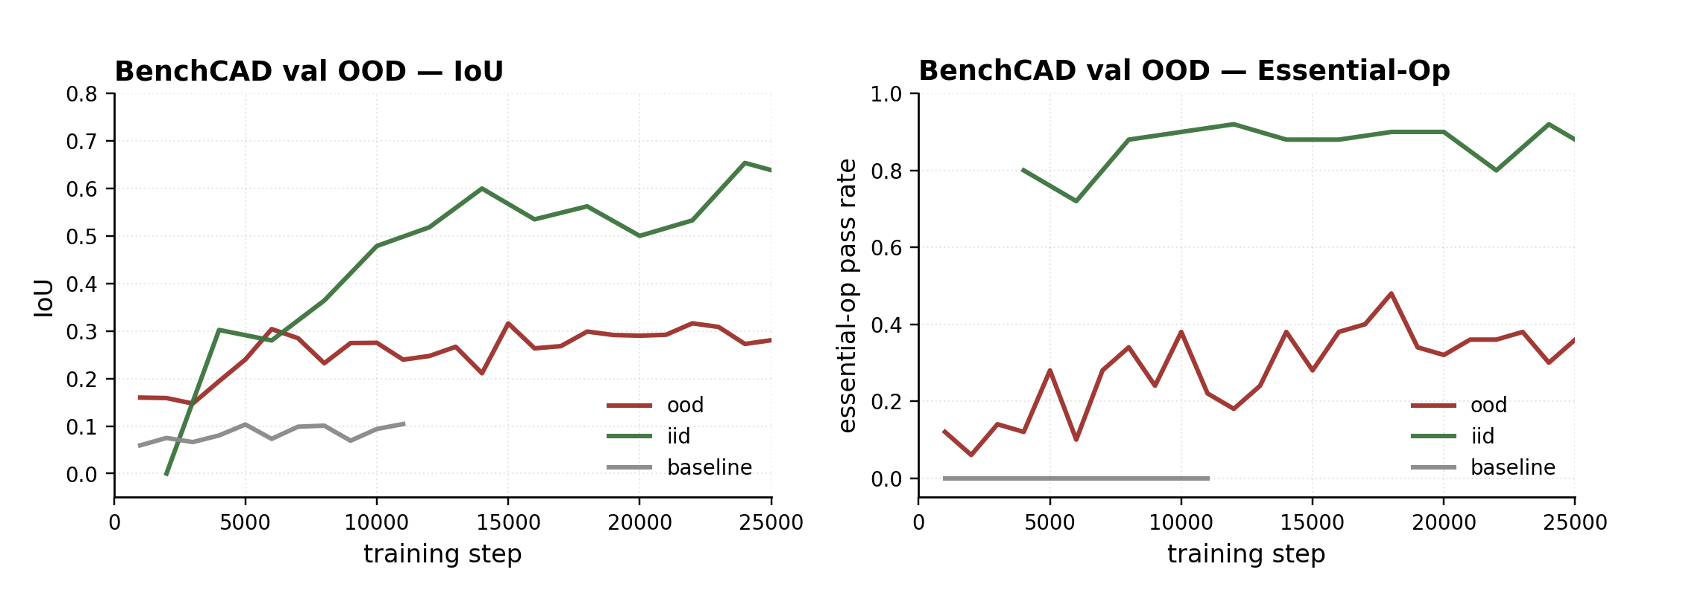
\includegraphics[width=0.85\linewidth]{figures/fig_7.png}
  \caption{\textbf{The generalisation gap on BenchCAD.} Qwen3-VL-2B trained on three data mixtures, evaluated on the BenchCAD validation set throughout training.
    \emph{(a) OOD IoU vs.\ training step.} The IID-trained run (green) climbs highest; the OOD run (red, trained without the held-out family slice) plateaus mid-range; the baseline (grey, no BenchCAD) stays near the floor.
    \emph{(b) OOD essential-op pass rate.} IID reaches the highest rate, OOD plateaus mid-range, baseline stays at $\sim$0\% --- the \textbf{CAD Operational Blindspot}.
    The deficit is not optimisation budget, not backbone capacity, and not training-corpus operation coverage alone --- it is the fundamental difficulty of constructing industry-grade parametric CAD code on \emph{unseen} family distributions.}
  \label{fig:generalisation_gap}
\end{figure*}
\section{Datasheet for BenchCAD}
\label{app:datasheet}

We follow the datasheet template of Gebru et al.\ (2021); responses below are condensed for the appendix and reproduced in full as a separate Croissant 1.0 metadata file shipped with the dataset release.

\paragraph{Motivation.}
\textbf{For what purpose was the dataset created?} BenchCAD was created to evaluate the parametric-CAD capabilities of large vision-language and code-language models along three sub-capabilities (visual perception, parametric abstraction, code synthesis) on industrially representative part families with execution-verified ground truth.
\textbf{Who created the dataset and on behalf of which entity?} The authors. (Anonymised for double-blind submission.)
\textbf{Who funded the dataset?} The authors' individual funds. (Anonymised.)

\paragraph{Composition.}
\textbf{What do the instances represent?} Each instance is a parametric CAD part: an executable CadQuery Python program, the resulting STEP file, four canonical-view PNG renders, a parameter JSON, and an op-list JSON.
\textbf{How many instances are there in total?} 17{,}900 verified parts in BenchCAD, 2{,}400 paired QA questions in BenchCAD-QA (each evaluated under both visual and code conditioning, yielding 4{,}800 records), and 748 curated edit pairs in BenchCAD-Edit.
\textbf{Does the dataset contain all possible instances?} No --- BenchCAD samples a subset of all the industry CAD generation part familys, and sampled a subset of parameter space per family; the schema permits unbounded sampling under the documented constraints.
\textbf{Is there a label/target?} The CadQuery source code, STEP, parameters, and op list jointly serve as ground truth; for QA tasks, gold answers are derived deterministically from parameters; for edit tasks, target code and target STEP are paired with the original.

\paragraph{Collection process.}
\textbf{How was the data acquired?} Procedurally generated by the BenchCAD generation pipeline (\S\ref{sec:dataset}); the only human-in-the-loop component is edit-pair curation by the authors.
\textbf{Who was involved in data collection?} The authors.
\textbf{Were any ethical review processes conducted?} Not applicable; no human-subjects data.

\paragraph{Preprocessing/cleaning/labeling.}
\textbf{Was preprocessing/cleaning done?} Verification (sandbox execution + non-degenerate volume + 30\,s timeout, followed by domain-expert visual sign-off) is the sole filter applied to BenchCAD.
The Fusion360 and DeepCAD subsets undergo additional curation: parsing failures and parts whose reconstruction yields invalid geometry are excluded.
\textbf{Was the raw data saved?} Yes; the unverified pre-filter output is retained for analysis and is available on request.

\paragraph{Uses.}
\textbf{Has the dataset been used for any tasks already?} The five tasks defined in \S\ref{sec:tasks}.
\textbf{Is there anything that prevents responsible reuse?} The dataset contains no PII, no copyrighted source designs, and no safety-sensitive specifications.
The standard-anchored families reference public ISO/DIN/EN/ASME/IEC standard codes by number and name; we do not redistribute the standard documents themselves.

\paragraph{Distribution.}
\textbf{Will the dataset be distributed?} Yes, on Hugging Face under \texttt{BenchCAD/cad\_bench} and \texttt{BenchCAD/cad\_bench\_edit}.
\textbf{When?} On submission acceptance (or on arXiv release if earlier).
\textbf{Under what licence?} CC-BY-4.0 for data; MIT for code (generation pipeline, evaluation harness, baseline checkpoint).
\textbf{Are there restrictions?} Standard CC-BY-4.0 attribution.

\paragraph{Maintenance.}
\textbf{Who will support the dataset?} The authors via the GitHub issue tracker and Hugging Face dataset card.
\textbf{How will errata be communicated?} Versioned releases on Hugging Face with changelogs in the dataset card.

\section{Question Bank Construction}
\label{app:qbank}

The numeric-QA tasks (\texttt{qa\_img}, \texttt{qa\_code}) draw from a per-family question bank constructed in three steps. (1) For each family, a domain-knowledge author writes 6--12 question \emph{templates} parameterised by the family's exposed parameters --- e.g.\ for \texttt{involute\_gear}: \emph{``what is the ratio of root-to-tip diameter?''}, \emph{``how many teeth does the visible gear have?''}.
Templates are typed (ratio, integer count, ordinal) and constrained to be scale-invariant. (2) Templates are instantiated per-record by deterministic substitution of the verified parameter values, yielding a gold answer alongside each question. (3) A second author reviews each instantiation for ambiguity and visibility (a question must be answerable from the four canonical views with no occluded features).
The final bank contains 2{,}400 unique (question, gold answer) pairs sampled across 17{,}900 records --- each evaluated under both visual (\texttt{qa\_img}) and code (\texttt{qa\_code}) conditioning, yielding 4{,}800 total QA records.
The composition is approximately 60\% ratio, 35\% integer count, and 5\% ordinal. We release the question-template source code so that the bank can be regenerated under alternative parameter samples.

\section{QA System Prompts}
\label{app:qa-system-prompts}

To ensure reproducibility, we provide the exact system prompts used in our QA evaluation.
All models are evaluated with the same prompt template. The model is required to output
only a JSON array of numbers, which enables automatic numeric grading. For binary
questions, we encode ``yes'' as 1 and ``no'' as 0.

\subsection{Image-based QA System Prompt}
\label{app:qa-img-system-prompt}

\begin{tcolorbox}[
    title=\texttt{QA\_IMG\_SYSTEM\_PROMPT},
    colback=gray!4,
    colframe=gray!45,
    fonttitle=\bfseries,
    breakable,
    sharp corners,
    boxrule=0.5pt,
]
\small
You are an expert CAD engineer. You will be shown a
\texttt{DIAGONAL\_VIEW\_LAYOUT}. You will be given a list of numeric
questions about the part. Answer each with a single number.

\vspace{0.5em}
\textbf{Rules:}
\begin{itemize}
    \item Output ONLY a JSON array of numbers, one per question, in the same order.
    \item No text, no keys, no explanation. Just the array.
    \item For yes/no questions, use 1 for yes and 0 for no.
    \item For count questions, use an integer, e.g., 12, not ``twelve''.
    \item For ratio questions, use a decimal, e.g., 2.5.
    \item For dimensional questions, answer in whatever consistent unit the code uses;
    the scale is arbitrary and the grader compares numeric magnitude.
\end{itemize}

\textbf{Example input:}
\begin{verbatim}
["How many teeth?", "What is the module?"]
\end{verbatim}

\textbf{Example output:}
\begin{verbatim}
[20, 2.5]
\end{verbatim}
\end{tcolorbox}

\subsection{Code-based QA System Prompt}
\label{app:qa-code-system-prompt}

\begin{tcolorbox}[
    title=\texttt{QA\_CODE\_SYSTEM\_PROMPT},
    colback=gray!4,
    colframe=gray!45,
    fonttitle=\bfseries,
    breakable,
    sharp corners,
    boxrule=0.5pt,
]

\small
You are an expert CAD engineer. You will be shown CadQuery Python code for a
mechanical part. You will be given a list of numeric questions about the part
this code produces.

\vspace{0.5em}
\textbf{Rules:}
\begin{itemize}
    \item Output ONLY a JSON array of numbers, one per question, in the same order.
    \item No text, no keys, no explanation. Just the array.
    \item For yes/no questions, use 1 for yes and 0 for no.
    \item For count questions, use an integer, e.g., 12, not ``twelve''.
    \item For ratio questions, use a decimal, e.g., 2.5.
    \item For dimensional questions, answer using the same scale as the numeric
    literals in the code.
\end{itemize}

\textbf{Example input code:} The code creates a gear with 20 teeth and module 2.5.

\textbf{Example input questions:}
\begin{verbatim}
["How many teeth in the gear?", "What is the module?"]
\end{verbatim}

\textbf{Example output:}
\begin{verbatim}
[20, 2.5]
\end{verbatim}
\end{tcolorbox}

\section{Code Generation System Prompts}
\label{app:codegen-system-prompts}

To ensure reproducibility, we provide the exact prompts used for code generation.
The model is given a normalized four-view composite render of an industrial part and
is asked to generate executable CadQuery Python code. All generated code is evaluated
under the same execution protocol: \texttt{cadquery} is pre-imported as \texttt{cq},
and the final reconstructed solid must be stored in \texttt{result}.

\subsection{Primary Vision-to-CAD System Prompt}
\label{app:primary-vision-to-cad-system-prompt}

\begin{tcolorbox}[
    title=\texttt{SYSTEM\_PROMPT},
    colback=gray!4,
    colframe=gray!45,
    fonttitle=\bfseries,
    breakable,
    sharp corners,
    boxrule=0.5pt
]
\small
Generate CadQuery Python code from a \texttt{DIAGONAL\_VIEW\_LAYOUT}.

\vspace{0.5em}
Renders are normalized: bbox centered at \texttt{[0.5,0.5,0.5]}, longest side maps to \texttt{[0,1]}.
Match the orientation exactly---do not rotate or remap axes. World XYZ in your code must match world XYZ in the renders.

\begin{itemize}
    \item \texttt{cadquery} is pre-imported as \texttt{cq}; no imports, no \texttt{show\_object}.
    \item Store final solid in \texttt{result}.
    \item Output ONLY code, no explanation or markdown.
\end{itemize}
\end{tcolorbox}

\subsection{Vision-to-CAD User Prompt}
\label{app:vision-to-cad-user-prompt}

\begin{tcolorbox}[
    title=\texttt{USER\_PROMPT},
    colback=gray!4,
    colframe=gray!45,
    fonttitle=\bfseries,
    breakable,
    sharp corners,
    boxrule=0.5pt
]
\small
Generate CadQuery code to recreate this industrial part shown in the 4-view composite render.
\end{tcolorbox}

\subsection{Cadrille Baseline System Prompt}
\label{app:cadrille-system-prompt}

\begin{tcolorbox}[
    title=\texttt{CADRILLE\_SYSTEM\_PROMPT},
    colback=gray!4,
    colframe=gray!45,
    fonttitle=\bfseries,
    breakable,
    sharp corners,
    boxrule=0.5pt
]
\small
You are a CadQuery expert. Given a normalized \texttt{DIAGONAL\_VIEW\_LAYOUT}.

\vspace{0.5em}
Write CadQuery Python code that reproduces the geometry. Output ONLY Python code.
\end{tcolorbox}


% \section{QA System Prompt}
% \label{app:qa_img_sys_prompt}

% \paragraph{QA\_IMG\_SYSTEM\_PROMPT}

% You are an expert CAD engineer. You will be shown a DIAGONAL\_VIEW\_LAYOUT. You will be given a list of numeric questions about the part. Answer each with a single number.

% Rules:\\
% - Output ONLY a JSON array of numbers, one per question, in the same order.\\
% - No text, no keys, no explanation. Just the array.\\
% - For yes/no questions, use 1 for yes and 0 for no.\\
% - For count questions, use an integer (e.g. 12, not "twelve").\\
% - For ratio questions, use a decimal (e.g. 2.5).\\
% - For dimensional questions, answer in whatever consistent unit the code uses (scale is arbitrary; the grader compares numeric magnitude).

% Example input: ["How many teeth?", "What is the module?"]\\
% Example output: [20, 2.5]

% \paragraph{QA\_CODE\_SYSTEM\_PROMPT}
% You are an expert CAD engineer. You will be shown CadQuery Python code for a mechanical part. You will be given a list of numeric questions about the part this code produces.

% Rules:
% - Output ONLY a JSON array of numbers, one per question, in the same order.\\
% - No text, no keys, no explanation. Just the array.\\
% - For yes/no questions, use 1 for yes and 0 for no.\\
% - For count questions, use an integer (e.g. 12, not "twelve").\\
% - For ratio questions, use a decimal (e.g. 2.5).\\
% - For dimensional questions, answer using the same scale as the numeric literals in the code.

% Example input code creates a gear with 20 teeth and module 2.5.
% Example input questions: ["How many teeth?", "What is the module?"]\\
% Example output: [20, 2.5]

\subsection{Edit-task System Prompt}
\label{app:edit-code-system-prompt}
\begin{tcolorbox}[title=\texttt{EDIT\_CODE\_SYSTEM\_PROMPT}, colback=gray!4, colframe=gray!45,fonttitle=\bfseries, breakable, sharp corners, boxrule=0.5pt,]                                   
  \small                                                         
  You are an expert CAD engineer. You will be given:
  \begin{enumerate}                                                   \item A CadQuery Python script that builds a parametric mechanical part.
      \item A natural-language edit instruction describing a change to one specific feature.                
  \end{enumerate}
    
  Your task: return the script with the MINIMAL edit that achieves the requested feature change. Only the feature(s) the instruction explicitly mentions should change; every other feature, dimension, and detail must stay exactly as in the original.    
  \vspace{0.5em}                                                  \textbf{Rules:}
  \begin{itemize}
  \item Output ONLY executable Python code, no explanation, no markdown fences.
  \item Make the smallest set of changes that realize the instruction. Do NOT touch unrelated literals, operations, or structure.
  \item Do NOT refactor, rename variables, reorder operations, or add/remove imports.
  \item If the instruction adds a new feature: append the operation in the most natural place; keep the rest of the chain intact.
  \item If the instruction removes a feature: delete just that operation block; do not rewrite surrounding code.
  \item If the instruction modifies a dimension/parameter: update only the literal(s) that depend on it (and, if present, the matching parameter comment).
  \end{itemize}
  \end{tcolorbox}                                                 
  
\label{app:edit-img-gt-system-prompt}                             \begin{tcolorbox}[
title=\texttt{EDIT\_IMG\_GT\_SYSTEM\_PROMPT},               
colback=gray!4, colframe=gray!45, fonttitle=\bfseries, breakable, sharp corners, boxrule=0.5pt,]
  \small
  You are an expert CAD engineer. You will be given:              
  \begin{enumerate}
  \item A CadQuery Python script that builds a parametric mechanical part(CURRENT state).
  \item A 2$\times$2 composite image of the TARGET geometry from 4 diagonal viewpoints.                                         
  \end{enumerate}                                                
  Your task: return the script with the MINIMAL edit that transforms the CURRENT geometry (described by the code) into the TARGET geometry (shown in the image). The image is the only specification of the desired change, there is NO text instruction. Compare the code's geometry against the image and infer which single feature differs.                      
  Only the feature(s) that differ between code and image should change; every other feature, dimension, and detail must stay exactly as in the original code.
    
  \vspace{0.5em}
  \textbf{Rules:}                                                               
  \begin{itemize}
  \item Output ONLY executable Python code, no explanation, no markdown fences.
  \item Make the smallest set of changes that realize the visual difference. Do NOT touch unrelated literals, operations, or structure.
  \item Do NOT refactor, rename variables, reorder operations, or add/remove imports.
  \item If the target image shows a new feature that is absent in the code: append the operation in the most natural place; keep the rest of the chain intact.
  \item If the target image shows a feature removed: delete just that operation block; do not rewrite surrounding code.
  \item If a dimension/parameter has changed: update only the literal(s) that control that dimension (and the matching parameter comment if present).  
  \end{itemize}
  \end{tcolorbox} 



\label{app:edit-img-system-prompt}

\begin{tcolorbox}[
    title=\texttt{EDIT\_CODE\_IMG\_SYSTEM\_PROMPT (Ablation)},
    colback=gray!4,
    colframe=gray!45,
    fonttitle=\bfseries,
    breakable,
    sharp corners,
    boxrule=0.5pt,
]
\small
You are an expert CAD engineer. You will be given:
\begin{enumerate}
    \item A CadQuery Python script that builds a parametric mechanical part.
    \item A natural-language edit instruction describing a change to one specific feature.
    \item A 2$\times$2 composite image of the part from 4 diagonal viewpoints (CURRENT state) as an additional visual reference for the script.
\end{enumerate}

Your task: return the script with the MINIMAL edit that achieves the
requested feature change. Only the feature(s) the instruction explicitly
mentions should change; every other feature, dimension, and detail must
stay exactly as in the original.

\vspace{0.5em}
\textbf{Rules:}
\begin{itemize}
    \item Output ONLY executable Python code, no explanation, no markdown fences.
    \item Make the smallest set of changes that realize the instruction. Do NOT touch unrelated literals, operations, or structure.
    \item Do NOT refactor, rename variables, reorder operations, or add/remove imports.
    \item If the instruction adds a new feature: append the operation in the most natural place; keep the rest of the chain intact.
    \item If the instruction removes a feature: delete just that operation block; do not rewrite surrounding code.
    \item If the instruction modifies a dimension/parameter: update only the literal(s) that depend on it (and, if present, the matching parameter comment).
\end{itemize}
\end{tcolorbox}




\section{Rotation-Invariant IoU}
\label{app:iou}

We compute IoU under a configurable rotation-invariant protocol, taking the maximum over either the 6-element face-up cube symmetry group or the full 24-element cube rotation group. Before voxelization, each part is normalized by centering it at the origin and scaling it by the largest semi-axis of its bounding box. For each candidate rotation $g \in G$, we rotate the predicted voxel grid $\hat{V}$ and compute its overlap with the reference voxel grid $V$; the reported score is
\[
\max_{g \in G} \mathrm{IoU}(g \cdot \hat{V}, V).
\]
This metric is used diagnostically rather than as the primary score: a large gain from standard IoU to 24-rotation IoU indicates that the model may have generated the right geometry on the wrong construction plane. This failure is partly induced by a workplane prior: in online database, and manufacturing-oriented modeling workflows, parts are commonly initialized on the \texttt{XY} plane as the default sketching or setup plane. As a result, models may over-prefer \texttt{XY}-based constructions even when the target geometry is defined on \texttt{XZ} or \texttt{YZ}. Consistent with this interpretation, Table~\ref{tab:rot24_base_plane} shows substantially larger rotation-IoU gains for \texttt{XZ}/\texttt{YZ} ground-truth parts than for \texttt{XY} parts.
\begin{table}[t]
\centering
\small
\setlength{\tabcolsep}{6pt}
\renewcommand{\arraystretch}{1.08}
\caption{\textbf{Effect of rotation-invariant IoU by GT base plane.}
For GPT-4o, we report $\Delta=\mathrm{IoU}_{\mathrm{rot24}}-\mathrm{IoU}_{\mathrm{single\text{-}axis}}$ over 164 valid 24-IoU samples with extrusion. Larger $\Delta$ indicates cases where the generated shape is geometrically similar but expressed in a mismatched coordinate frame.}
\label{tab:rot24_base_plane}
\begin{tabular}{@{}lrrrr@{}}
\toprule
GT base plane & $n$ & Mean $\Delta$ & Max $\Delta$ \\
\midrule
XY  & 70  & 0.0463 & 0.5907 \\
XZ  & 40  & 0.2305 & 0.8031 \\
YZ  & 54  & 0.2140 & 0.7053 \\
\bottomrule
\end{tabular}
\end{table}

\section{Edit Protocol}
\label{app:edit_protocol}

\paragraph{Pair construction.} The 748 BenchCAD-Edit pairs are drawn balanced across 106 families and four edit categories (balanced across dimensional, additive, subtractive, and multi-step categories).
For each pair, we (i) start from a verified BenchCAD record, (ii) apply a parameter or op-list edit yielding a target part, (iii) verify the target satisfies the same verification pipeline, (iv) write a natural-language instruction by template (\emph{``increase the bore diameter to 12\,mm''}) reviewed for unambiguity by a second author, and (v) cross-validate by running two strong models and inspecting any unexpected failure modes.
Pairs where models systematically disagree on instruction interpretation are revised or removed.

\paragraph{Scoring.} See Eq.~\ref{eq:edit_acc} for metric definitions (normalised IoU used in edit-task score). The non-target preservation check is computed on the spatial complement of the bounding region of the targeted feature (precomputed bounding-box annotation per pair).


\paragraph{Task taxonomy.} The five edit task types (T1--T5) are defined in Table~\ref{tab:task_taxonomy}. Difficulty rises monotonically with the structural complexity of the minimal correct diff, from a single literal swap (T1) to coordinated multi-block restructures (T5). The T1--T5 axis is orthogonal to the dimensional/additive/subtractive/multi-step categorisation used in the main paper: T1 and T3 are predominantly dimensional, T2 and T4 cover additive/subtractive, and T5 spans the multi-step regime.

\begin{table}[t]
\centering
\caption{\textbf{BenchCAD-Edit task taxonomy.} The 748 edit pairs are stratified into five task types T1--T5 by the structural form of the minimal correct diff. Difficulty rises monotonically from T1 (one-literal swap) to T5 (multi-block restructure with trig or coordinated sub-feature changes).}
\label{tab:task_taxonomy}
\small
\begin{tabular}{@{}p{0.04\linewidth}p{0.18\linewidth}p{0.30\linewidth}p{0.18\linewidth}p{0.20\linewidth}@{}}
\toprule
\textbf{Code} & \textbf{Name} & \textbf{Definition} & \textbf{Diff signature} & \textbf{Example instruction} \\
\midrule
T1 & literal\_replace & Replace a single numeric literal that the instruction names explicitly (\emph{from X to Y}). & one literal swap; equal lines added/removed & \emph{``Increase the cylinder radius from 4.5 to 5.85.''} \\
T2 & chain\_transform & Append a single chainable whole-part transform (rotate / mirror / array). & one \texttt{result = result.<op>(...)} line appended & \emph{``Rotate the entire part by 90 degrees about the X axis.''} \\
T3 & relative\_compute & Read an existing literal and derive another value (ratio, percentage, $2\times$, $1/4$). & one literal swap, value derived from another literal & \emph{``Set the central bore diameter equal to twice the hub-cylinder height.''} \\
T4 & feature\_edit & Add or delete a single CSG sub-block (hole, slot, recess, chamfer, fillet, boss). & one 3--7 line CSG block inserted or removed & \emph{``Drill a 6 diameter through-hole along the Z axis.''} \\
T5 & geometry\_rebuild & Non-trivial restructure: trig-derived slopes/chamfers/lofts, or paragraph-style rebuilds where two or more sub-features change in concert. & multi-block rewrite, trig in code, paragraph instruction & \emph{``Replace the ramped arms and raised center with a single flat cross-shaped solid of uniform thickness.''} \\
\bottomrule
\end{tabular}
\end{table}



\paragraph{Failure taxonomy.} Every failing prediction is bucketed into one of eight semantic failure modes F01--F08 (Table~\ref{tab:failure_codes}), each mapped to one of the four capability layers L1--L4: F01--F03 isolate L1 \emph{Holistic Visual Understanding} (wrong value, wrong instance, wrong placement), F04--F06 isolate L2 \emph{CAD Operations Comprehension} (wrong axis, wrong selector, near no-op), F07 isolates L3 \emph{Industrial Parametric Abstraction} (incomplete multi-instance update), and F08 isolates L4 \emph{Spatial Reasoning $+$ Code Synthesis} (compositional geometry mismatch). Each label combines an automatic detection cue --- execution status, generated-vs-original/target IoU thresholds, and topology checks with a hand audit by the authors against the predicted code and rendered geometry; the rule set and L-mapping are fixed across all ten models reported, and \texttt{ok} (strict pass) and \texttt{exec\_fail} are tracked separately as the non-failure and gross-execution categories.

\begin{table}[t]
\centering
\caption{\textbf{Failure-mode taxonomy (F-codes).} Eight semantic failure modes used in the per-model failure analysis (Fig.~\ref{fig:edit_F_bars}). Each F-code is mapped to one capability layer: L1 \emph{Holistic Visual Understanding}, L2 \emph{CAD Operations Comprehension}, L3 \emph{Industrial Parametric Abstraction}, L4 \emph{Spatial Reasoning $+$ Code Synthesis}. Hand-labelled on the failing predictions of every BenchCAD-Edit run.}
\label{tab:failure_codes}
\small
\setlength{\tabcolsep}{4pt}
\renewcommand{\arraystretch}{1.15}
% allow line breaks at underscores in fixed-width name cells
\newcommand{\fname}[1]{\seqsplitfallback{#1}}
\providecommand{\seqsplitfallback}[1]{#1}
\begin{tabular}{@{}p{0.06\linewidth}p{0.18\linewidth}p{0.28\linewidth}p{0.18\linewidth}p{0.18\linewidth}@{}}
\toprule
\textbf{Code} & \textbf{Name} & \textbf{Definition} & \textbf{Detection cue} & \textbf{Representative failure} \\
\midrule
F01 \mbox{(L1)} & wrong\_\allowbreak param\_\allowbreak value & Right operation, wrong numerical value: dim, diameter, radius, length, or angle written off-target; geometry shape-correct but a single number misses. & $\mathrm{IoU}_{\text{gen}} \geq 0.9$, output differs from target by a single literal. & Model writes radius $5.6$ when prompt asks for $5.85$; cylinder topology unchanged. \\
F02 \mbox{(L1)} & wrong\_\allowbreak feature\_\allowbreak instance & Among multiple similar features (front vs.\ back ring, two legs, several circles), the model edits the wrong one or perturbs a neighbour. & $\mathrm{IoU}_{\text{gen}}$ swings markedly above OR below baseline; topology preserved. & Edit asks to enlarge the rear bore; model enlarges the front bore. \\
F03 \mbox{(L1)} & wrong\_\allowbreak placement & Right operation and value, but feature placed at slightly wrong coordinate, face, or orientation. & $\mathrm{IoU}_{\text{gen}} \geq 0.95$, small rigid offset against target. & Hole drilled $2$\,mm off-centre on a face whose origin the model misread. \\
F04 \mbox{(L2)} & wrong\_\allowbreak axis\_\allowbreak or\_\allowbreak direction & Rotation, mirror, or extrude direction wrong: rotate axis tuple permuted, mirror plane misidentified, sweep tangent flipped. & \texttt{status==ok}; rotated/mirrored bbox mismatches target axis. & gpt-4o rotate: \texttt{rotate((axis), (origin), deg)} with first two args swapped. \\
F05 \mbox{(L2)} & wrong\_\allowbreak selector\_\allowbreak or\_\allowbreak face & \texttt{.faces()}/\texttt{.edges()} selector returns wrong subset: \texttt{>Y} chosen on a Z-up part, OR-selector returns multi-face, lofted-face selector silently misses. & \texttt{status==ok}; operation applied to wrong topology vs.\ target. & Chamfer applied to all top edges instead of the single outer rim. \\
F06 \mbox{(L2)} & near\_\allowbreak no\_\allowbreak op\_\allowbreak under\_\allowbreak edit & Output $\approx$ original: comment-only edit, deleted wrong line, retained the feature meant to be removed, or applied the edit with no observable geometric effect. & $|\mathrm{IoU}_{\text{gen}} - \mathrm{IoU}_{\text{orig}}| < 0.005$. & claude-opus-4-7 (no-think): on $49\%$ of the failed records that rewrites the original byte-for-byte. \\
F07 \mbox{(L3)} & incomplete\_\allowbreak multi\_\allowbreak update & Edit requires updating multiple symmetric or repeated instances (helical-sweep points, replicated bolts/legs); model updates only a subset. & $\mathrm{IoU}_{\text{gen}}$ plateaus below $1.0$ across attempts; partial symmetry break. & Cross-parameter dim asks to scale all four legs; model scales only two. \\
F08 \mbox{(L4)} & compositional\_\allowbreak geometry\_\allowbreak mismatch & Composite or structural shape (slope strip, loft, sweep cross-section, multi-feature reorganisation) is partially right but does not match GT topology. & \texttt{status==ok}; $\mathrm{IoU}_{\text{gen}} \in [0.4, 0.95]$ on a T5-style edit. & Slope edit produces a chamfer of correct angle but along the wrong face strip. \\
\bottomrule
\end{tabular}
\end{table}



\paragraph{Image-conditioned variant.} To probe whether the textual instruction itself is a confound --- i.e.\ whether models succeed because the instruction states the change explicitly rather than because they reason about the geometry --- we additionally evaluate an image-conditioned setting in which the natural-language instruction is replaced by a four-view render of the target solid (\texttt{EDIT\_IMG\_GT\_SYSTEM\_PROMPT}, Appendix~\ref{app:edit-img-gt-system-prompt}); the model receives the original code and must infer the edit visually. Across the four OpenAI models we tested, \texttt{mean\_norm} drops by $0.40$--$0.85$\,pt at every task type (Fig.~\ref{fig:edit_image_type}). The dominant failure mode is that a render specifies geometry but not numbers: the model can usually tell whether a feature is added or removed (T2/T4 retain weak signal), but cannot recover the exact dimension a textual ``from $X$ to $Y$'' would have stated, so dimensional edits (T1, T3) collapse to near-zero and trig-driven rebuilds (T5) floor uniformly at $0$. Image-only conditioning is therefore a strict lower bound on the text protocol and, in its current form, primarily isolates feature-presence reasoning rather than parametric exactness.

                                               

\paragraph{Supplementary results.} Figure~\ref{fig:edit_F_bars} reports failure attributes of all 748 eidt-pairs from 10 LLMs.
Figure~\ref{fig:edit_L_pies} disaggregates per-model failures into the L1--L4 buckets defined in Figure~\ref{fig:capability_hierarchy}. Figure~\ref{fig:edit_image_type} reports the parallel image-based setting (target render in lieu of an NL instruction) broken down by T1--T5.

\begin{figure}[t]                       
    \centering
    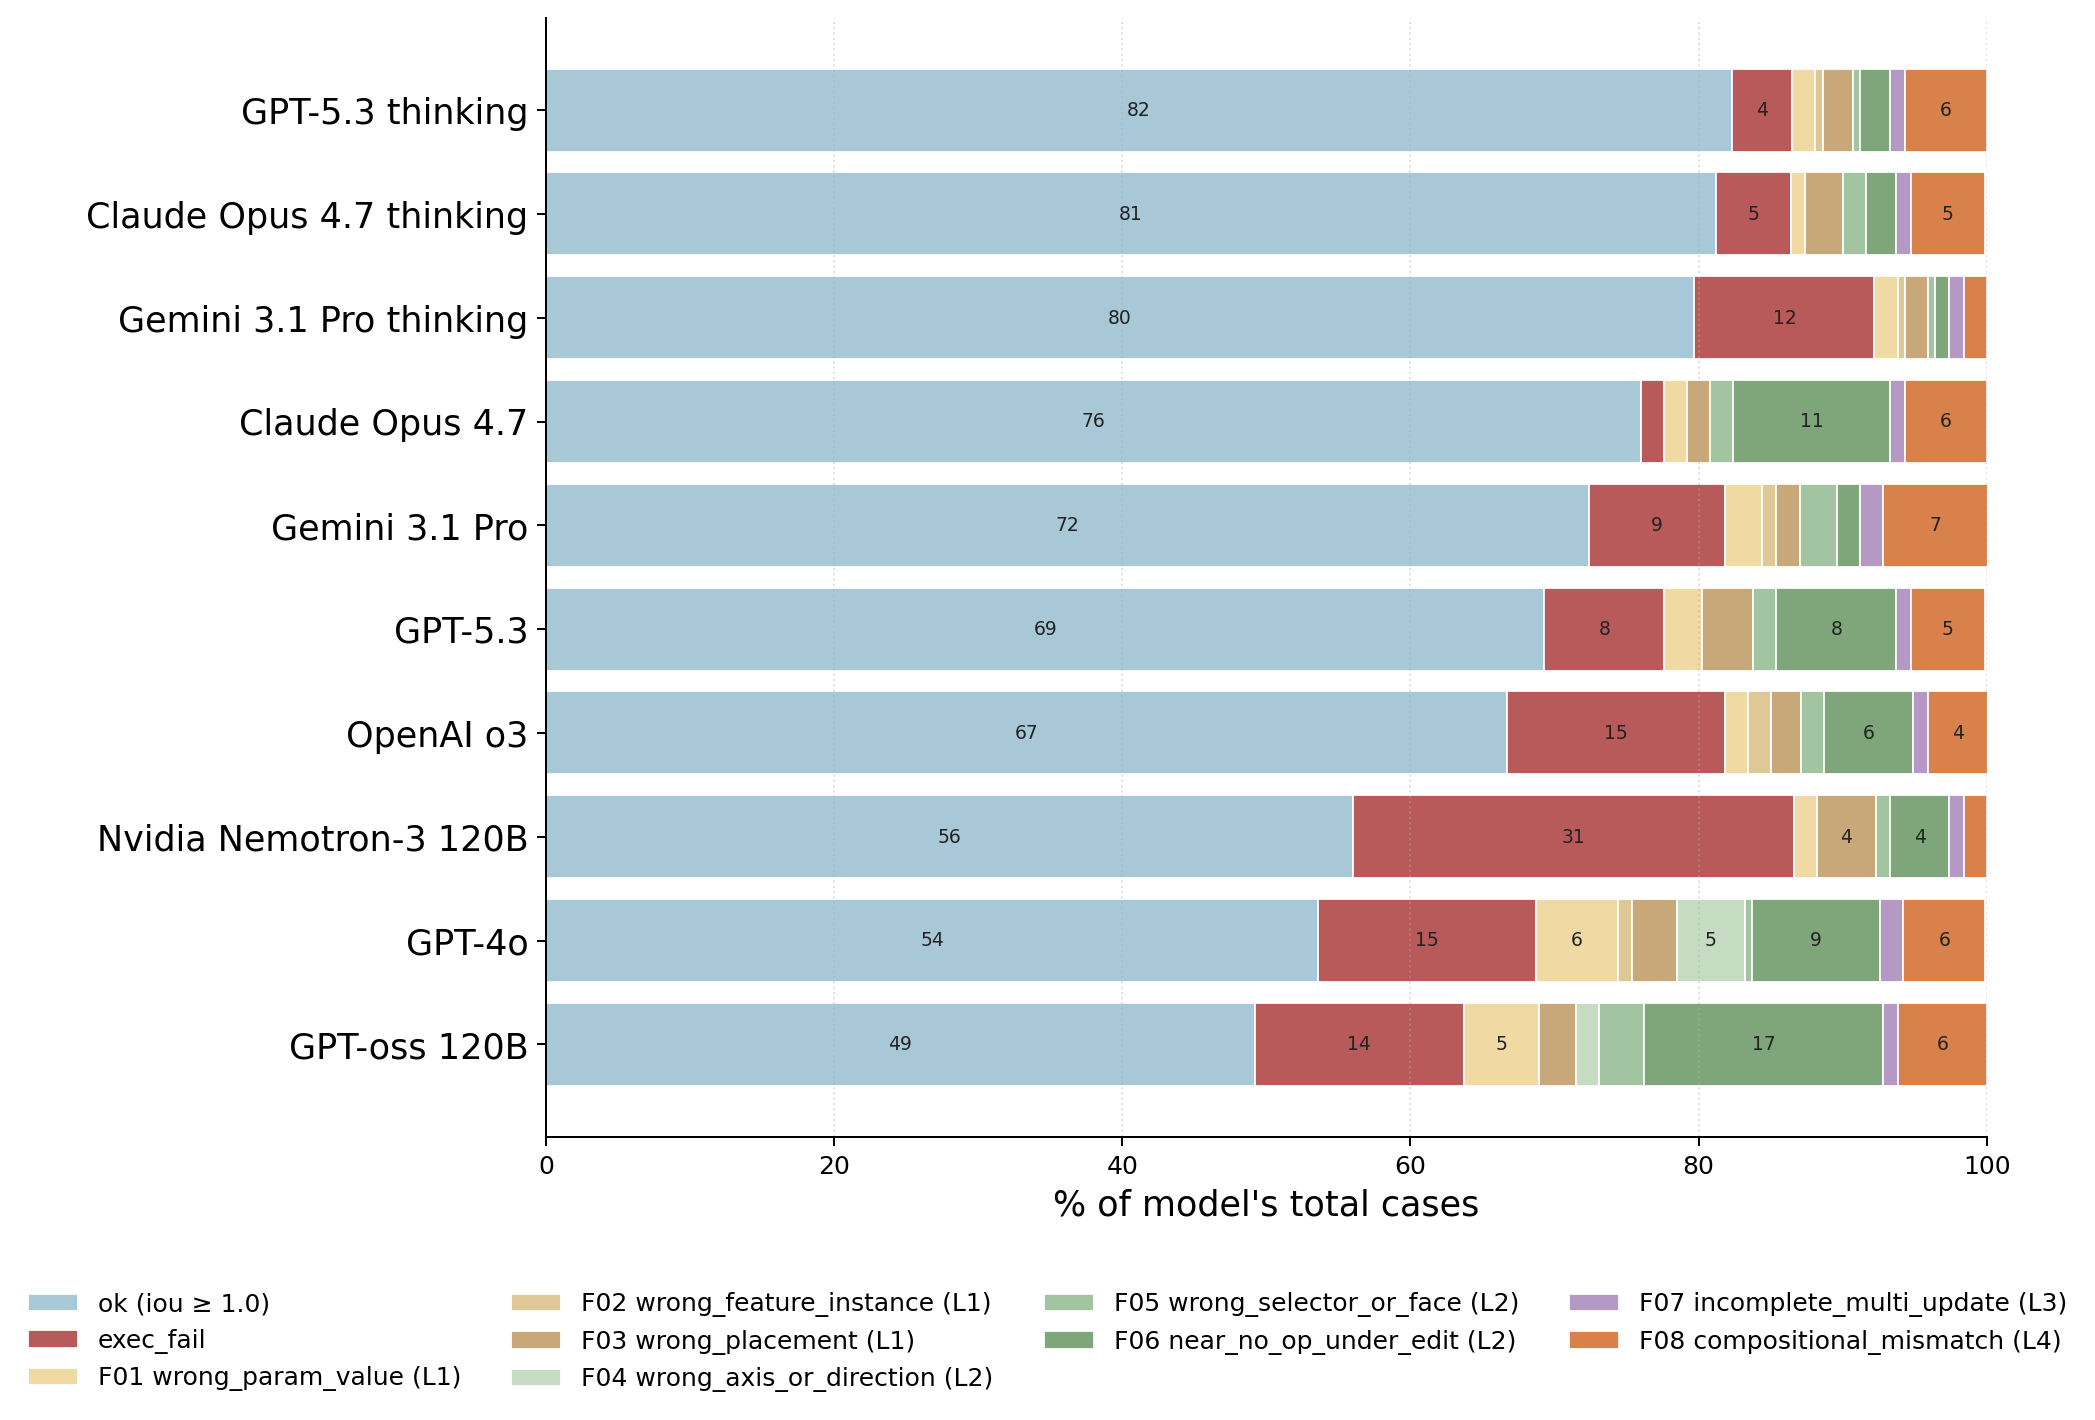
\includegraphics[width=0.95\linewidth]{figures/fig_F_bars.png}
    \caption{\textbf{Per-model failure-mode distribution on BenchCAD-Edit.} Each
   horizontal bar disaggregates one model's predictions into \texttt{ok},
  \texttt{exec\_fail}, and the eight semantic failure modes F01--F08 defined in 
  Table~\ref{tab:failure_codes}; segments are coloured by the underlying
  capability layer (sand $=$ L1 \emph{Holistic Visual Understanding}, sage $=$  
  L2 \emph{CAD Operations Comprehension}, purple $=$ L3 \emph{Industrial
  Parametric Abstraction}, orange $=$ L4 \emph{Spatial Reasoning $+$ Code       
  Synthesis}), so the L-mass within each bar reads off directly. Models are
  ordered by \texttt{ok} rate. The mass shifts systematically across model    
  generations: older or smaller-capacity systems concentrate failures in the L2
  band (F04--F06) and incur a non-trivial \texttt{exec\_fail} tail; recent large
   models without explicit reasoning largely close the L2 gap and leave residual
   mass on L1 (F01--F03); reasoning-tier closed models flatten L1 and L2 alike
  but expose an L3--L4 ceiling (F07--F08) on multi-instance and T5-style
  coordinated edits, indicating that thinking lifts capability up the
  L-hierarchy rather than uniformly reducing all error types.}
    \label{fig:edit_F_bars}
  \end{figure}  

\begin{figure}[t]
  \centering
  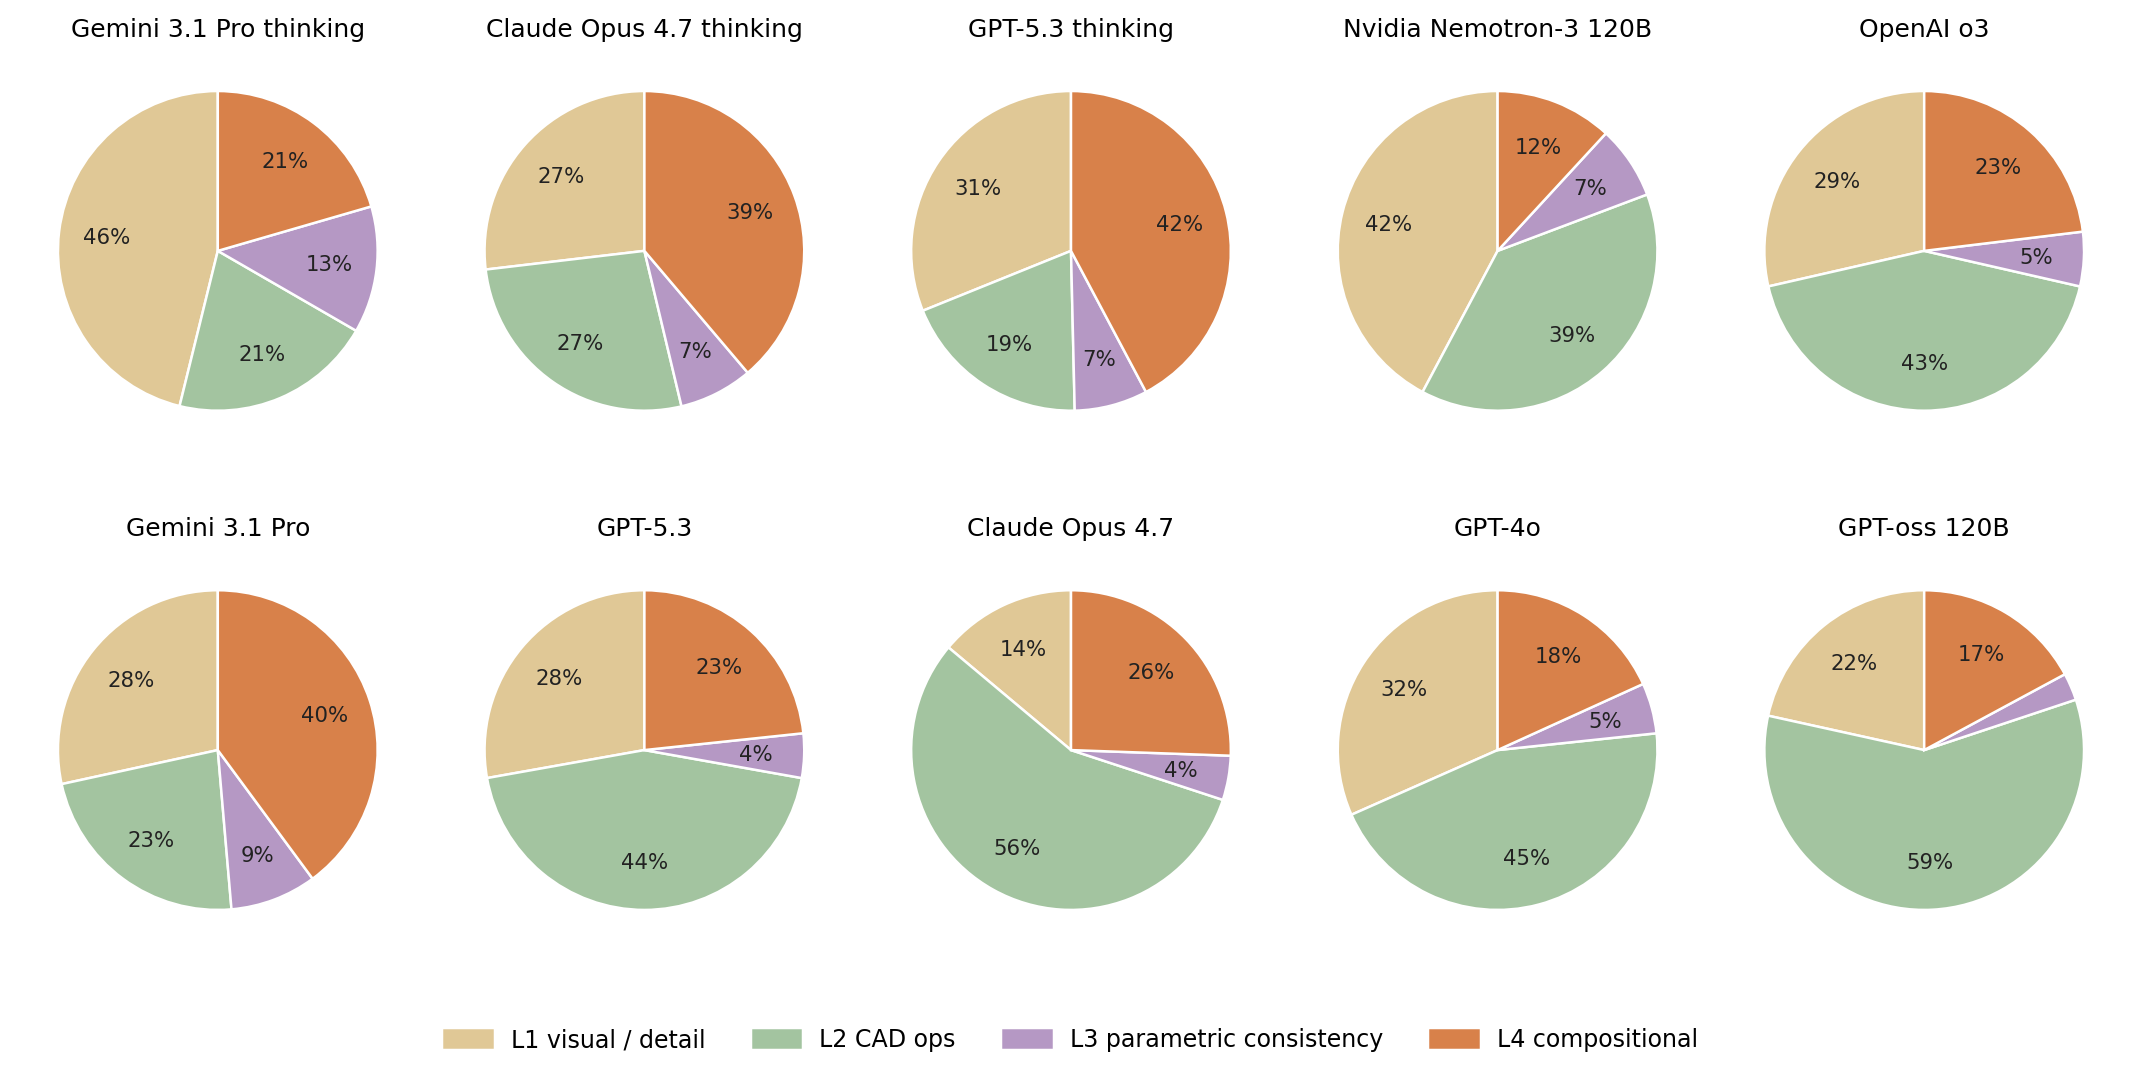
\includegraphics[width=0.95\linewidth]{figures/fig_L_pies.png}
  \caption{\textbf{Per-model failure-layer distribution on BenchCAD-Edit.} Each pie shows one model's failures aggregated by capability layer L1--L4 (collapsing the eight F-codes via the mapping in Table~\ref{tab:failure_codes}: F01--F03 $\to$ L1, F04--F06 $\to$ L2, F07 $\to$ L3, F08 $\to$ L4) and re-normalised so L1$+$L2$+$L3$+$L4 $= 100\%$ --- i.e.\ the pies show the \emph{shape} of each model's failure mode mix, independent of how often it fails overall; the title above each pie reports the absolute L-fail rate (\% of all predictions) so that scale is preserved. Models are arranged in order of increasing total L-fail rate (least-broken first). The mass shifts systematically along the L-axis across model generations: older or smaller-capacity systems concentrate failures in L2 (CAD-API misuse) and incur a non-trivial \texttt{exec\_fail} tail (counted separately, not shown); recent large models without explicit reasoning largely close the L2 gap and leave residual mass on L1 (visual/detail mistakes); reasoning-tier closed models flatten L1 and L2 alike but expose an L3--L4 ceiling on multi-instance and T5-style coordinated edits, indicating that thinking lifts capability up the L-hierarchy rather than uniformly reducing all error types.}
  \label{fig:edit_L_pies}
\end{figure}

\begin{figure}[t]
  \centering
  
\includegraphics[width=0.95\linewidth]{neurips_2026/figures/fig_edit_image_type.png}
  \caption{\textbf{Text vs.\ image conditioning.} Same $100$-pair subset, four OpenAI models, two protocols: \emph{text} sees the original code plus a natural-language instruction, \emph{image} replaces the instruction with a four-view render of the target solid (\texttt{EDIT\_IMG\_GT\_SYSTEM\_PROMPT}, App.~\ref{app:edit-img-gt-system-prompt}). Bars are \texttt{mean\_norm} (Eq.~\eqref{eq:edit_acc}) per task type. Text dominates uniformly, with the largest gaps at T1 and T3: a render shows what the part should look like but never tells the model that a radius is $5.85$, so dimensional edits collapse. T2 and T4 retain weak image signal because adding or removing a feature is something a render can communicate. T5 floors at zero either way. Reasoning helps the text side substantially but barely moves the image side, so current chain-of-thought mostly strengthens code-side reasoning rather than visual diff inference. Image-only conditioning is a strict lower bound on the text protocol; in its current form it primarily probes feature-presence reasoning, not parametric exactness.}
  \label{fig:edit_image_type}
\end{figure}


\section{Scoring-Protocol Ablations}
\label{app:ablation}

\begin{table}[t]
\centering
\small
\caption{\textbf{Scoring-protocol and inference-strategy ablations.} Reported on GPT-5.3 (think) on BenchCAD-Lite. Removing scale invariance (allowing absolute mm hints in prompts) inflates \texttt{qa\_img} by 4.6\,pt --- the systematic optimism baked into prior CAD-eval protocols. Best-of-5 sampling and multi-turn refinement with execution feedback offer diminishing-returns improvements. Doubling view count from 4 to 8 closes only $\leq$1.5\,pt of the Holistic Spatial and Detailing Deficit, far below what a perception bottleneck would predict.}
\label{tab:ablation}
\begin{tabular}{lrr}
\toprule
Variant & Avg & $\Delta$ \\
\midrule
GPT-5.3 full (4-view img + scale-invariant prompts) & 46.8 & -- \\
$-$ single front view only                        & 38.5 & $-$8.3 \\
$+$ 8-view grid (vs.\ 4-view)                     & 47.6 & $+$0.8 \\
$-$ scale-invariant prompts (mm hints leak)       & 51.4 & $+$4.6 (inflated) \\
$-$ rotation-invariant IoU (axis-aligned only)    & 40.9 & $-$5.9 (under-credited) \\
$+$ Best-of-5 sampling                            & 52.1 & $+$5.3 \\
$+$ multi-turn refinement w/ exec feedback (3 turns) & 55.8 & $+$9.0 \\
\bottomrule
\end{tabular}
\end{table}


Table~\ref{tab:ablation} reports two scoring-protocol ablations on the Vision2Code task. (i) The \emph{24-axial vs.\ single-axis IoU} contrast quantifies how much credit is recovered by accounting for wrong-plane outputs (\S\ref{sec:exp_failure_analysis}, $L_1$ spatial-anchoring failure mode): when the gap is large, the model's geometry is approximately correct but emitted on a non-canonical workplane. (ii) The \emph{single-view vs.\ multi-view} contrast quantifies how much of a model's score is driven by the four-view evidence specifically, isolating the cost of removing back-side and depth cues from the perception input.

\section{CadQuery Operation Coverage}
\label{app:ops}

\begin{table}[t]
\centering
\small
\caption{\textbf{CadQuery operation coverage versus prior corpora.} BenchCAD covers 28 distinct operations spanning primitives, 2D sketching, advanced solid ops (helical sweeps, lofts, shells), boolean composition, holes, arrays, and finishing features. Prior CAD datasets are largely restricted to sketch + extrude.}
\label{tab:op_coverage}
\begin{tabular}{lccccccc}
\toprule
Bench & sk+ex & rev. & loft/sw. & bool. & fil/cham & twistEx. & spline/helix \\
\midrule
DeepCAD              & \cmark & --     & --     & basic  & --     & --     & --     \\
Text2CAD             & \cmark & --     & --     & --     & --     & --     & --     \\
CAD-Coder            & \cmark & --     & --     & --     & --     & --     & --     \\
CAD-Recode (1M)      & \cmark & --     & --     & \cmark & --     & --     & --     \\
CADPrompt (200)      & \cmark & part.  & part.  & \cmark & --     & --     & --     \\
CADEvolve            & \cmark & \cmark & --     & \cmark & part.  & --     & --     \\
\midrule
\textbf{BenchCAD}    & \cmark & \cmark & \cmark & \cmark & \cmark & \cmark & \cmark \\
\bottomrule
\end{tabular}
\end{table}


Table~\ref{tab:op_coverage} reports the per-category breakdown.

\paragraph{Static analysis protocol.}
For each released CadQuery corpus we extract distinct method invocations using the regex \texttt{$\backslash$.([A-Za-z\_]\textbackslash w*)(} on the \texttt{.py} text. We then EXCLUDE three groups: (a) class/type names (\texttt{Workplane}, \texttt{Vector}, \texttt{Wire}, \texttt{Solid}, \texttt{Sketch}, \texttt{Compound}, \texttt{Edge}, \texttt{Face}, \texttt{Plane}, \texttt{Location}, \texttt{Shape}, \texttt{Edges}, \texttt{Vertices}); (b) selectors / accessors that do not modify geometry (\texttt{face}, \texttt{faces}, \texttt{edges}, \texttt{vertices}, \texttt{wires}, \texttt{val}, \texttt{vals}, \texttt{first}, \texttt{last}, \texttt{tag}, \texttt{newObject}, \texttt{copyWorkplane}, \texttt{plane}); and (c) Python stdlib / numpy / utility helpers (\texttt{append}, \texttt{join}, \texttt{format}, \texttt{sin}, \texttt{cos}, \texttt{multiply}, \ldots). The same EXCLUDE list is applied uniformly across BenchCAD, CADEvolve seeds, CAD-Recode/cadrille, GenCAD-Code, and CADPrompt. Saturation curves: CAD-Recode at $1{,}274$ \texttt{.py} (op count constant from $200$ files onward); GenCAD-Code at $2{,}000$ streamed samples (constant from $100$ samples onward).

\paragraph{Tier B (sketch+extrude IR works).}
DeepCAD, Fusion360 Gallery, and Text2CAD release a tokenized intermediate representation rather than executable CadQuery, so the CadQuery static-analysis rule does not apply directly. We instead report the IR's primitive-token alphabet: DeepCAD encodes parts as \{\texttt{L}, \texttt{A}, \texttt{C}, \texttt{EXT}\} plus two control tokens \{\texttt{SOL}, \texttt{EOS}\} (\citet{Wu2021}, Sec.~3); Fusion360 Gallery r1.0.1 specifies $8$ sketch curve types (\texttt{SketchLine}, \texttt{SketchArc}, \texttt{SketchCircle}, \texttt{ConicCurve}, \texttt{Ellipse}, \texttt{EllipticalArc}, \texttt{FittedSpline}, \texttt{FixedSpline}) plus extrude with $4$ boolean variants \citep{Willis2021fusion}; Text2CAD reuses the CAD-SIGNet tokenizer ($\sim$$17$-token alphabet over end-of-X markers, quantized coords, and $4$ extrude booleans). These counts are not directly comparable to method counts on CadQuery \texttt{.py} releases; in Table~\ref{tab:cmp_prior} we accordingly summarize each work as \emph{narrow} (sketch+extrude IR or a small CadQuery subset) or \emph{broad} (wide CadQuery API).

\paragraph{CADEvolve caveat.}
CADEvolve's Hugging Face release (\texttt{kulibinai/cadevolve}, $\sim$$2$M rows, $4.7$\,GB) contains only \texttt{.npy} sentence embeddings keyed by component name, not Python source. The full $\sim$$1.3$M expanded scripts are referenced in the paper but are not part of the public release. We therefore report CADEvolve's operation count from the $46$ hand-written seed programs in \texttt{evolution/cadquery\_examples.txt} of the GitHub repo \texttt{zhemdi/CADEvolve}, yielding $30$ distinct ops --- a strict lower bound on the full evolved corpus.

\section{Reproduction Recipe}
\label{app:reproduce}

Reproduction uses the released \texttt{bench/fetch\_data.py} (Hugging Face fetch), the \texttt{bench.eval} runner (\texttt{--model <model> --task <task> --seed 42}), and each released model's documented inference entry-point.
We provide adapter wrappers under \texttt{bench/models/providers/} for cadrille and CADEvolve so that the existing runner accepts these models without modification.
Per-task IoU, Chamfer distance, execution rate, and per-family breakdowns are exported to \texttt{results/<task>/<model>/}.
For training the open BenchCAD baseline: \texttt{train/sft\_qwen3vl.py} with the released training config and data manifest.

\clearpage
\section{Ethical Considerations and Broader Impact}
\label{app:ethics}

BenchCAD contains procedurally generated parametric CAD parts and references public engineering standards by code and name.
The dataset contains no personal data, no proprietary designs, and no safety-sensitive specifications.
Potential risks of CAD-capable models more broadly --- e.g.\ accelerated reverse-engineering of regulated components --- are not specific to BenchCAD and are best addressed at the model-deployment layer rather than the benchmark layer.
We see no negative societal impact specific to this work that is not already present in the underlying open-source CAD ecosystem.


\newpage

\clearpage
\section*{NeurIPS Paper Checklist}

\begin{enumerate}

\item {\bf Claims}
    \item[] Question: Do the main claims made in the abstract and introduction accurately reflect the paper's contributions and scope?
    \item[] Answer: \answerYes{}
    \item[] Justification: The abstract and \S\ref{sec:intro} state three contributions (BenchCAD dataset and CadGen pipeline; capability-decomposed task suite including the first verified parametric edit task; the Holistic Spatial and Detailing Deficit / CAD Operational Blindspot / Industrial Common Sense and Parametric Abstraction Gap diagnostics). Each claim is substantiated in \S\ref{sec:dataset}--\S\ref{sec:results} with experimental results on 10+ models.

\item {\bf Limitations}
    \item[] Question: Does the paper discuss the limitations of the work performed by the authors?
    \item[] Answer: \answerYes{}
    \item[] Justification: Appendix~\ref{app:limitations} is a dedicated Limitations section discussing the standard-parametric-vs-industrial-CAD gap, the standard-anchored-vs-compliant distinction, and the bounded scope of the Industrial Common Sense Gap measurement.

\item {\bf Theory assumptions and proofs}
    \item[] Question: For each theoretical result, does the paper provide the full set of assumptions and a complete (and correct) proof?
    \item[] Answer: \answerNA{}
    \item[] Justification: The paper presents an empirical benchmark and dataset; it makes no theoretical claims requiring proofs.

    \item {\bf Experimental result reproducibility}
    \item[] Question: Does the paper fully disclose all the information needed to reproduce the main experimental results of the paper to the extent that it affects the main claims and/or conclusions of the paper (regardless of whether the code and data are provided or not)?
    \item[] Answer: \answerYes{}
    \item[] Justification: \S\ref{sec:experiments} lists the 10+ evaluated models, decoding settings, and per-task scoring; Appendix~\ref{app:reproduce} provides the reproduction recipe (data fetch command, runner invocation, adapter wrappers, training config). Dataset, code, and baseline checkpoint are released under permissive licences.


\item {\bf Open access to data and code}
    \item[] Question: Does the paper provide open access to the data and code, with sufficient instructions to faithfully reproduce the main experimental results, as described in supplemental material?
    \item[] Answer: \answerYes{}
    \item[] Justification: All BenchCAD splits are released on Hugging Face (\texttt{BenchCAD/cad\_bench}, \texttt{BenchCAD/cad\_bench\_edit}) under CC-BY-4.0; the CadGen pipeline, evaluation harness, and BenchCAD-trained baseline checkpoint are released under MIT. Appendix~\ref{app:reproduce} gives exact commands.


\item {\bf Experimental setting/details}
    \item[] Question: Does the paper specify all the training and test details (e.g., data splits, hyperparameters, how they were chosen, type of optimizer) necessary to understand the results?
    \item[] Answer: \answerYes{}
    \item[] Justification: \S\ref{sec:exp_setup} specifies the evaluation settings; \S\ref{sec:exp_training} specifies the open BenchCAD-trained baseline's training recipe (Qwen3-VL-2B; SFT three splits + GRPO). Appendix~\ref{app:reproduce} provides the runner commands and points to the released training config.

\item {\bf Experiment statistical significance}
    \item[] Question: Does the paper report error bars suitably and correctly defined or other appropriate information about the statistical significance of the experiments?
    \item[] Answer: \answerNo{}
    \item[] Justification: All reported numbers are single-seed evaluations due to the cost of running 10+ models including proprietary APIs. We report per-family stratification (Table~\ref{tab:family_cliff}) so variance can be assessed across difficulty tiers. Future releases will include multi-seed error bars for the open BenchCAD-trained baseline.

\item {\bf Experiments compute resources}
    \item[] Question: For each experiment, does the paper provide sufficient information on the computer resources (type of compute workers, memory, time of execution) needed to reproduce the experiments?
    \item[] Answer: \answerYes{}
    \item[] Justification: \S\ref{sec:exp_setup} describes inference compute; \S\ref{sec:exp_training} describes baseline training; Appendix~\ref{app:reproduce} provides the runner invocation.

\item {\bf Code of ethics}
    \item[] Question: Does the research conducted in the paper conform, in every respect, with the NeurIPS Code of Ethics?
    \item[] Answer: \answerYes{}
    \item[] Justification: The dataset is procedurally generated, contains no PII or proprietary designs, and references public engineering standards by code only. No human-subjects data is collected.


\item {\bf Broader impacts}
    \item[] Question: Does the paper discuss both potential positive societal impacts and negative societal impacts of the work performed?
    \item[] Answer: \answerYes{}
    \item[] Justification: Appendix~\ref{app:ethics} discusses the dataset's lack of personal or proprietary content, the potential dual-use risk inherent to any improved CAD-capable model, and the absence of negative impacts specific to BenchCAD beyond those of the broader open-source CAD ecosystem.

\item {\bf Safeguards}
    \item[] Question: Does the paper describe safeguards that have been put in place for responsible release of data or models that have a high risk for misuse?
    \item[] Answer: \answerNA{}
    \item[] Justification: BenchCAD contains expert-authored parametric CAD parts referencing public engineering standards. The released open baseline (Qwen3-VL-2B) poses no high-risk misuse potential beyond what is already available in open-source CAD ecosystems.

\item {\bf Licenses for existing assets}
    \item[] Question: Are the creators or original owners of assets used in the paper properly credited and are the license and terms of use explicitly mentioned and properly respected?
    \item[] Answer: \answerYes{}
    \item[] Justification: We credit DeepCAD~\citep{Wu2021}, Fusion360 Gallery~\citep{Willis2021fusion}, Qwen2-VL~\citep{Qwen2VL}, and the cadrille/CADEvolve checkpoints with explicit licence statements. Re-distribution of derived data complies with the source licences.

\item {\bf New assets}
    \item[] Question: Are new assets introduced in the paper well documented and is the documentation provided alongside the assets?
    \item[] Answer: \answerYes{}
    \item[] Justification: BenchCAD ships with a Croissant 1.0 metadata file (validated by the public Croissant checker), per-family parameter schemas, dataset card, and the datasheet of Appendix~\ref{app:datasheet}. The CadGen pipeline and evaluation harness include README, environment specification, and reproduction commands.

\item {\bf Crowdsourcing and research with human subjects}
    \item[] Question: For crowdsourcing experiments and research with human subjects, does the paper include the full text of instructions given to participants and screenshots, if applicable, as well as details about compensation (if any)?
    \item[] Answer: \answerYes{}
    \item[] Justification: BenchCAD does not involve human-subjects evaluation; the dataset is procedurally generated and all reported metrics are computed by automated execution and verification pipelines.

\item {\bf Institutional review board (IRB) approvals or equivalent for research with human subjects}
    \item[] Question: Does the paper describe potential risks incurred by study participants, whether such risks were disclosed to the subjects, and whether Institutional Review Board (IRB) approvals (or an equivalent approval/review based on the requirements of your country or institution) were obtained?
    \item[] Answer: \answerNA{}
    \item[] Justification: The only human-subjects component is paid professional CAD engineers scoring CAD samples on a standard consulting basis; no personal data is collected and no risk to participants beyond ordinary professional work. IRB review is not required by the authors' institutions for this engagement type.

\item {\bf Declaration of LLM usage}
    \item[] Question: Does the paper describe the usage of LLMs if it is an important, original, or non-standard component of the core methods in this research?
    \item[] Answer: \answerYes{}
    \item[] Justification: LLMs are the evaluated subjects, not core method components. Where LLMs assist in dataset construction (e.g., GPT-5-mini in CADEvolve's evolutionary expansion, used here only as a transfer baseline), this is described in \S\ref{sec:exp_training}. The CadGen procedural pipeline contains no LLM in the loop. LLM use in writing assistance is incidental.

\end{enumerate}


\end{document}
